\batchmode
\makeatletter
\def\input@path{{\string"P:/IMD/Karl/New Trustee Orientation 2017/\string"}}
\makeatother
\documentclass[10pt,english]{beamer}\usepackage[]{graphicx}\usepackage[]{color}
%% maxwidth is the original width if it is less than linewidth
%% otherwise use linewidth (to make sure the graphics do not exceed the margin)
\makeatletter
\def\maxwidth{ %
  \ifdim\Gin@nat@width>\linewidth
    \linewidth
  \else
    \Gin@nat@width
  \fi
}
\makeatother

\definecolor{fgcolor}{rgb}{0.345, 0.345, 0.345}
\newcommand{\hlnum}[1]{\textcolor[rgb]{0.686,0.059,0.569}{#1}}%
\newcommand{\hlstr}[1]{\textcolor[rgb]{0.192,0.494,0.8}{#1}}%
\newcommand{\hlcom}[1]{\textcolor[rgb]{0.678,0.584,0.686}{\textit{#1}}}%
\newcommand{\hlopt}[1]{\textcolor[rgb]{0,0,0}{#1}}%
\newcommand{\hlstd}[1]{\textcolor[rgb]{0.345,0.345,0.345}{#1}}%
\newcommand{\hlkwa}[1]{\textcolor[rgb]{0.161,0.373,0.58}{\textbf{#1}}}%
\newcommand{\hlkwb}[1]{\textcolor[rgb]{0.69,0.353,0.396}{#1}}%
\newcommand{\hlkwc}[1]{\textcolor[rgb]{0.333,0.667,0.333}{#1}}%
\newcommand{\hlkwd}[1]{\textcolor[rgb]{0.737,0.353,0.396}{\textbf{#1}}}%
\let\hlipl\hlkwb

\usepackage{framed}
\makeatletter
\newenvironment{kframe}{%
 \def\at@end@of@kframe{}%
 \ifinner\ifhmode%
  \def\at@end@of@kframe{\end{minipage}}%
  \begin{minipage}{\columnwidth}%
 \fi\fi%
 \def\FrameCommand##1{\hskip\@totalleftmargin \hskip-\fboxsep
 \colorbox{shadecolor}{##1}\hskip-\fboxsep
     % There is no \\@totalrightmargin, so:
     \hskip-\linewidth \hskip-\@totalleftmargin \hskip\columnwidth}%
 \MakeFramed {\advance\hsize-\width
   \@totalleftmargin\z@ \linewidth\hsize
   \@setminipage}}%
 {\par\unskip\endMakeFramed%
 \at@end@of@kframe}
\makeatother

\definecolor{shadecolor}{rgb}{.97, .97, .97}
\definecolor{messagecolor}{rgb}{0, 0, 0}
\definecolor{warningcolor}{rgb}{1, 0, 1}
\definecolor{errorcolor}{rgb}{1, 0, 0}
\newenvironment{knitrout}{}{} % an empty environment to be redefined in TeX

\usepackage{alltt}
\usepackage{mathptmx}
\usepackage[T1]{fontenc}
\usepackage[latin9]{inputenc}
\usepackage{babel}
\usepackage{array}
\usepackage{amsmath}
\usepackage{amssymb}
\usepackage{graphicx}
\usepackage{setspace}
\ifx\hypersetup\undefined
  \AtBeginDocument{%
    \hypersetup{unicode=true}
  }
\else
  \hypersetup{unicode=true}
\fi

\makeatletter

%%%%%%%%%%%%%%%%%%%%%%%%%%%%%% LyX specific LaTeX commands.
%% Because html converters don't know tabularnewline
\providecommand{\tabularnewline}{\\}

%%%%%%%%%%%%%%%%%%%%%%%%%%%%%% Textclass specific LaTeX commands.
 % this default might be overridden by plain title style
 \newcommand\makebeamertitle{\frame{\maketitle}}%
 % (ERT) argument for the TOC
 \AtBeginDocument{%
   \let\origtableofcontents=\tableofcontents
   \def\tableofcontents{\@ifnextchar[{\origtableofcontents}{\gobbletableofcontents}}
   \def\gobbletableofcontents#1{\origtableofcontents}
 }

%%%%%%%%%%%%%%%%%%%%%%%%%%%%%% User specified LaTeX commands.


\usetheme{Warsaw}
%
%start of text to add page numbers
%
\setbeamercolor{mycolor}{fg=white,bg=black}
\defbeamertemplate*{footline}{shadow theme}{%
\leavevmode%
\hbox{\begin{beamercolorbox}[wd=.5\paperwidth,ht=2.5ex,dp=1.125ex,leftskip=.3cm plus1fil,rightskip=.3cm]{author in head/foot}%
    \usebeamerfont{author in head/foot}\hfill\insertshortauthor
\end{beamercolorbox}%
\begin{beamercolorbox}[wd=.4\paperwidth,ht=2.5ex,dp=1.125ex,leftskip=.3cm,rightskip=.3cm plus1fil]{title in head/foot}%
    \usebeamerfont{title in head/foot}\insertshorttitle\hfill%
\end{beamercolorbox}%
\begin{beamercolorbox}[wd=.1\paperwidth,ht=2.5ex,dp=1.125ex,leftskip=.3cm,rightskip=.3cm plus1fil]{mycolor}%
\hfill\insertframenumber\,/\,\inserttotalframenumber
\end{beamercolorbox}}%
\vskip0pt%
}
%
%end of text to add page numbers
%


%\setbeamercovered{transparent}
% or whatever (possibly just delete it)


%
%below removes navigation symbols
%you might want this is a version for live presentation
\setbeamertemplate{navigation symbols}{}
%\setbeamertemplate{footline}[page number]

%
%sets the page size a little bigger to get more text in a default font size
\geometry{paperwidth=141mm,paperheight=106mm} 

%comment out next two lines for screen viewing with active hyperlinks 
\usepackage{pgfpages}
\pgfpagesuselayout{resize to}[letterpaper,border shrink=5mm,landscape]

%
%hyperlink settings
%
%\usepackage{hyperref}
%\hypersetup{colorlinks=true,citecolor=green}
\definecolor{links}{HTML}{2A1B81}
\hypersetup{colorlinks,linkcolor=,urlcolor=links}

\makeatother
\IfFileExists{upquote.sty}{\usepackage{upquote}}{}
\begin{document}




\title{Investment Management}

\date[2017]{2017}

\author{Arizona State Retirement System}

\makebeamertitle
\AtBeginSection[]{%
  \frame<beamer>{ 
    \frametitle{Outline}   
    \tableofcontents[currentsection,currentsubsection] 
  }
}
\AtBeginSubsection[]{%
  \frame<beamer>{ 
    \frametitle{Outline}   
    \tableofcontents[currentsection,currentsubsection] 
  }
}


\section{Investment Management Division Overview}

\subsection{Introduction}
\begin{frame}{Introduction}
\begin{itemize}
\item ASRS is responsible for the administration of \$36 billion in assets
in connection with the retirement plan and other related activities
\item The Investment Management Division (``IMD'') manages these assets
\item In this document, we will describe the investment program and the
processes to implement and govern the program
\end{itemize}
\end{frame}
%
\begin{frame}{IMD Tasks and Responsibilities}
\begin{itemize}
\item Operate the investment program
\begin{itemize}
\item Manage internal portfolios of stocks and bonds
\item Search for and diligize external asset managers 
\item Monitor external managers
\end{itemize}
\item Evaluate performance using returns and holdings based techniques 
\item Monitor markets and portfolio composition for rebalance and tactical
positioning opportunities
\item Research and strategy formulation on both macro and micro dimensions
\item Prepare various reports for internal use, the board and the public
\item Operate a compliance system to ensure all legal and policy requirements
are met
\end{itemize}
\end{frame}

\begin{frame}{Investment Goals}
\begin{itemize}
\item We describe our investment program in terms of assets, strategy and
process
\begin{itemize}
\item We make market returns by owning assets
\item We enhance those returns by strategies and processes designed to add
value
\end{itemize}
\item Our goal is to invest in a well diversified portfolio designed to
earn attractive returns considering the risks taken
\item By following this strategy, the portfolio is structured to earn above
market returns and to earn the actuarially assumed rate of return
over a long horizon 
\end{itemize}
\end{frame}
%

\subsection{Assets}
\begin{frame}{Strategic Asset Allocation}
\begin{itemize}
\item ASRS invests in accordance with a strategic asset allocation (``SAA'')
policy
\item The SAA is updated not less frequently than once every four years
\item The current SAA provides the following target allocations:
\begin{itemize}
\item Equities 58\%, including
\begin{itemize}
\item Domestic equities 26\%
\item Developed and Emerging Market International Equities 24\%
\item Private Equity 8\%
\end{itemize}
\item Credit and lending strategies 14\%, including
\begin{itemize}
\item Private Debt 12\%
\item High Yield 2\%
\end{itemize}
\item Interest Rate Sensitive Fixed Income 11\%
\item Real Estate 10\%
\item Multi-asset class strategies 5\%
\item Commodities 2\%
\end{itemize}
\item The complete SAA can be found at \href{https://www.azasrs.gov/content/asset-allocation}{https://www.azasrs.gov/content/asset-allocation}
\end{itemize}
\end{frame}
%
\begin{frame}{Risk and Return}
\begin{itemize}
\item The SAA is designed to provide a well diversified portfolio across
multiple return generation sources
\begin{itemize}
\item {\footnotesize{}We think of ``return generation source'' and ``risk''
as synonymous} 
\end{itemize}
\item In order to make money, you have to take risk
\item We think of risk primarily in terms of business risk, i.e.
\begin{itemize}
\item {\footnotesize{}The ability of companies to successfully sell products
and manage their operations}{\footnotesize \par}
\item {\footnotesize{}The ability of properties to attract tenants}{\footnotesize \par}
\item {\footnotesize{}The ability of borrowers to repay their loans when
we extend them credit}{\footnotesize \par}
\end{itemize}
\item The economy, business cycle and capital markets dynamics also are
a source of risk
\begin{itemize}
\item {\footnotesize{}The economy has ups and downs creating risks and opportunities}{\footnotesize \par}
\item {\footnotesize{}Economic retractions are a source of risk, particularly
for enterprises lacking resources to ride out a recession}{\footnotesize \par}
\item {\footnotesize{}Unanticipated inflation is a risk for fixed rate investments
and for businesses which may need time to adjust to changing prices}{\footnotesize \par}
\item {\footnotesize{}When investors seek safety during a recession this
causes the prices of risky assets to decline, particularly if stressed
or illiquid parties become compelled sellers}{\footnotesize \par}
\item {\footnotesize{}This is a source of opportunity for investors who
are long term oriented and have the resources and fortitude to take
advantage of these opportunities}{\footnotesize \par}
\end{itemize}
\end{itemize}
\end{frame}
%
\begin{frame}{Market Returns}
\begin{itemize}
\item ASRS engages in the strategic asset allocation process in order to
define and place constraints on the broad categories of assets we
will own
\begin{itemize}
\item We invest in businesses through stocks and private equity
\begin{itemize}
\item This is a globally diversified portfolio across market capitalization
and including both developed and emerging economies
\end{itemize}
\item We invest in government and investment grade bonds where the source
of return is primarily related to interest rates
\item We invest in ``credit'', i.e. loans to companies where the return
derives primarily spreads to risk free interest rates
\item We invest in properties, primarily commercial real estate but also
agriculture and infrastructure
\item We invest in commodities, currencies and other liquid assets where
the source of return may be driven by ``alternative risk premia'' 
\end{itemize}
\item We benchmark returns from these assets against market indices of comparable
type and risk
\item Sometimes, market returns from assets are called ``beta''
\end{itemize}
\end{frame}
%

\subsection{Strategy}
\begin{frame}{Trading in Efficient Markets}
 
\begin{itemize}
\item Generally, listed markets are quite efficient and very hard to beat
\item Nevertheless, even the most liquid markets offer trading opportunities
which we systematically explore and exploit in our internal portfolios.
For example, 
\begin{itemize}
\item There is some predictability in price patterns around index name changes
\item There may be opportunity for larger investors to profit by providing
liquidity for block trades
\item Futures may at times be ``cheap'' providing enhanced return opportunities
\item Capital market dynamics may influence the pricing of risk and create
investment opportunity across fixed income sectors
\end{itemize}
\end{itemize}
\end{frame}
%
\begin{frame}{Idiosyncratic Risk and Information Advantage in Private Markets}
\begin{itemize}
\item {\footnotesize{}While listed markets generally are liquid and efficient
enough to arbitrage away any diversifiable idiosyncratic risk, private
markets operate differently because}{\footnotesize \par}
\begin{itemize}
\item {\footnotesize{}Information is widely and cheaply available in liquid
markets, while information is expensive and often proprietary in private
markets}{\footnotesize \par}
\item {\footnotesize{}It generally is illegal to trade on ``inside'' information
in liquid markets, while no such restriction applies to private markets}{\footnotesize \par}
\end{itemize}
\item {\footnotesize{}Diligence and information advantages}{\footnotesize \par}
\begin{itemize}
\item {\footnotesize{}We diligize asset managers to assess their skill,
process discipline and organizational depth}{\footnotesize \par}
\begin{itemize}
\item {\footnotesize{}We diligize markets, companies and properties when
investing directly}{\footnotesize \par}
\item {\footnotesize{}This method is most applicable in less liquid markets}{\footnotesize \par}
\item {\footnotesize{}Stock and bond markets are regulated so that investors
(and non-investors) have access to the same information; so, it is
generally not possible to gain an information edge in these markets}{\footnotesize \par}
\end{itemize}
\item {\footnotesize{}Business planning and strategy}{\footnotesize \par}
\begin{itemize}
\item {\footnotesize{}We invest in companies or properties with a plan in
mind and generate value by executing that plan}{\footnotesize \par}
\item {\footnotesize{}Requires long term orientation and control over management}{\footnotesize \par}
\item {\footnotesize{}Often requires specialized expertise in markets or
processes}{\footnotesize \par}
\end{itemize}
\end{itemize}
\item {\footnotesize{}Alignment of interest and avoidance of agency costs}{\footnotesize \par}
\begin{itemize}
\item {\footnotesize{}Invest in structures where management has the same
economic interest as investors }{\footnotesize \par}
\end{itemize}
\item {\footnotesize{}Collectively, these strategies allow us to pursue
idiosyncratic business risk and profit potential in private markets}{\footnotesize \par}
\end{itemize}
\end{frame}
%
\begin{frame}{Alternate Risk Premia in Equity and Other Markets}
 
\begin{itemize}
\item Alternate Risk Premia
\begin{itemize}
\item In liquid markets, there is strong evidence of risk factors driving
performance
\begin{itemize}
\item Fama and French demonstrate the influence of size and value on stock
performance in their research from the early 1990's
\item Additional research demonstrates additional factors such as carry
(yield) and momentum
\end{itemize}
\item These can be implemented in long only market portfolios such as the
ASRS risk factor portfolio
\item Or they can be implemented in long/short portfolios across multiple
markets with low correlation to those markets
\begin{itemize}
\item Investable directly or as an overlay to traditional beta 
\end{itemize}
\end{itemize}
\end{itemize}
\end{frame}
%
\begin{frame}{Gaining Performance Advantage as a Long Term Investor}
\begin{itemize}
\item Any investor with a large pool of capital in relation to their near
term needs is in a position to manage their assets to a longer horizon
\begin{itemize}
\item ASRS assets of \$36 billion are roughly 36 times the net annual outflow
for benefit payments
\end{itemize}
\item A long term investor can afford to be relatively indifferent to short
term ups and downs in its portfolio
\begin{itemize}
\item While ASRS measures and monitors volatility, we maintain focus on
the long term in order to gain advantage by a willingness to tolerate
short term market fluctuations
\end{itemize}
\item We ride out tough markets and do not sell risky assets in times of
stress
\item We rebalance in favor of risky assets when they fall below target
weights due to market action
\item We seek out opportunity to buy assets cheaply when they are impacted
by distress and market dislocations across a business cycle and due
to regulatory change
\end{itemize}
\end{frame}
%

\subsection{Processes}
\begin{frame}{Gaining Performance Advantage as a Tactical Investor}

\begin{itemize}
\item We monitor markets considering
\begin{itemize}
\item valuations relative to historic norms
\item relative valuation across asset classes
\item relative valuation of currency and global interest rates
\item trends and momentum
\end{itemize}
\item We document this analytical work in ``house views'' which are the
basis for tactical decisions to overweight or underweight certain
asset classes
\item A tactical positioning committee meets monthly (or more frequently
if necessary) to review and implement tactical decisions
\end{itemize}
\end{frame}
%
\begin{frame}{Strategy Formation and Idea Generation}

\begin{itemize}
\item The portfolio managers are experts in the markets they cover
\item They are responsible to monitor market conditions and identify opportunities
for attractive investment based capital markets dynamics, regulatory
dislocations and other factors leading to mispricing of risk
\item When a strategy for potential investment, the portfolio managers and
CIO concur on a plan for research and diligence which may culminate
in the deployment of capital 
\end{itemize}
\end{frame}
%
\begin{frame}{Research}
\begin{itemize}
\item We remain current in financial markets research as a source of ideas
for portfolio implementation
\item We conduct ongoing event studies and simulations as a source of ideas
for trading implementation in our internal portfolios
\end{itemize}
\end{frame}
%
\begin{frame}{Diligence}
\begin{itemize}
\item We engage in diligence in an effort to find the best partners and
business opportunities
\item In private markets we seek an information advantage through diligence
\item When our portfolio managers and research identify an opportunity
\begin{itemize}
\item we engage in an outbound process to find the best counterparties to
pursue the opportunity
\item we analyze their track record with state of the art statistical methods
\item we perform diligence on operational, organizational and legal matters
to confirm integrity in the implementation and conduct of their business
strategy
\end{itemize}
\end{itemize}
\end{frame}
%
\begin{frame}{Managing Liquidity}
\begin{itemize}
\item The annual net outflow for benefit payments is approximately \$1 billion
per year, compared to approximately \$36 billion in fund assets
\begin{itemize}
\item We have recurring cash flow from dividends, interest and rents which
can cover the preponderance of this negative cash flow without requirement
of asset sales
\end{itemize}
\item IMD manages liquidity to deliver cash to operating accounts when needed
for these payments
\item The bigger challenge is to ensure we have resources available to purchase
assets in times of stress and when they are cheap
\begin{itemize}
\item We maintain exposure to treasuries and investment grade bonds which
retain their value in such times 
\item We have flexibility to alter the ``beta'' allowing certain ``multi-asset''
strategies to operate as an overlay to other liquid assets, creating
an opportunity to increase exposure to stocks when warranted
\item We have structured our investments in less liquid sectors in separate
accounts that give us favorable liquidity terms and ability to control
investment pace if needed
\end{itemize}
\end{itemize}
\end{frame}
%
\begin{frame}{Performance Measurement and Feedback}
\begin{itemize}
\item We view performance measurement and feedback as an active part of
our investment process and not a mere administrative activity
\item Performance measurement adds value because you can only improve if
you are candid with yourself about what you are good at and where
you need to improve
\item In order to create the highest value from performance measurement,
the most advanced statistical methods are needed
\begin{itemize}
\item We implement both returns and holdings based analysis
\item and we are able to present that over varying time frames and rolling
periods in order to understand trends
\end{itemize}
\end{itemize}
\end{frame}
%
\begin{frame}{Cost Management}
\begin{itemize}
\item Costs matter and we are highly cognizant of costs in managing the
investment program
\begin{itemize}
\item We manage approximately one third of our assets internally at effectively
zero cost
\item The remainder of public market assets are managed with custom negotiated
vehicle and fee structures
\end{itemize}
\item Private market investments are generally implemented in strategies
involving highly specialized expertise 
\begin{itemize}
\item We need to acquire talent to pursue these strategies and cost minimization
is not the objective
\item We pursue high return on investment on any fees we pay
\begin{itemize}
\item by first diligizing managers and only negotiating with the most highly
qualified among them, and 
\item by structuring competitive negotiations among these managers
\end{itemize}
\item By implementing our private markets investment program largely through
separate accounts, we implement in much larger account sizes which
facilitates favorable negotiation of fees
\end{itemize}
\end{itemize}
\end{frame}
%

\subsection{Performance Summary}

\subsubsection{Total Fund}
\begin{frame}{Total Fund Returns}

\includegraphics[width=0.8\paperwidth,height=0.8\paperheight]{2P__IMD_Karl_R_projects_ASRS_TF_Return_asrs_returns.pdf}
\end{frame}
%

\subsubsection{Return Decomposition}
\begin{frame}[fragile]{10 Year Total Fund Return}

\begin{knitrout}
\definecolor{shadecolor}{rgb}{0.969, 0.969, 0.969}\color{fgcolor}
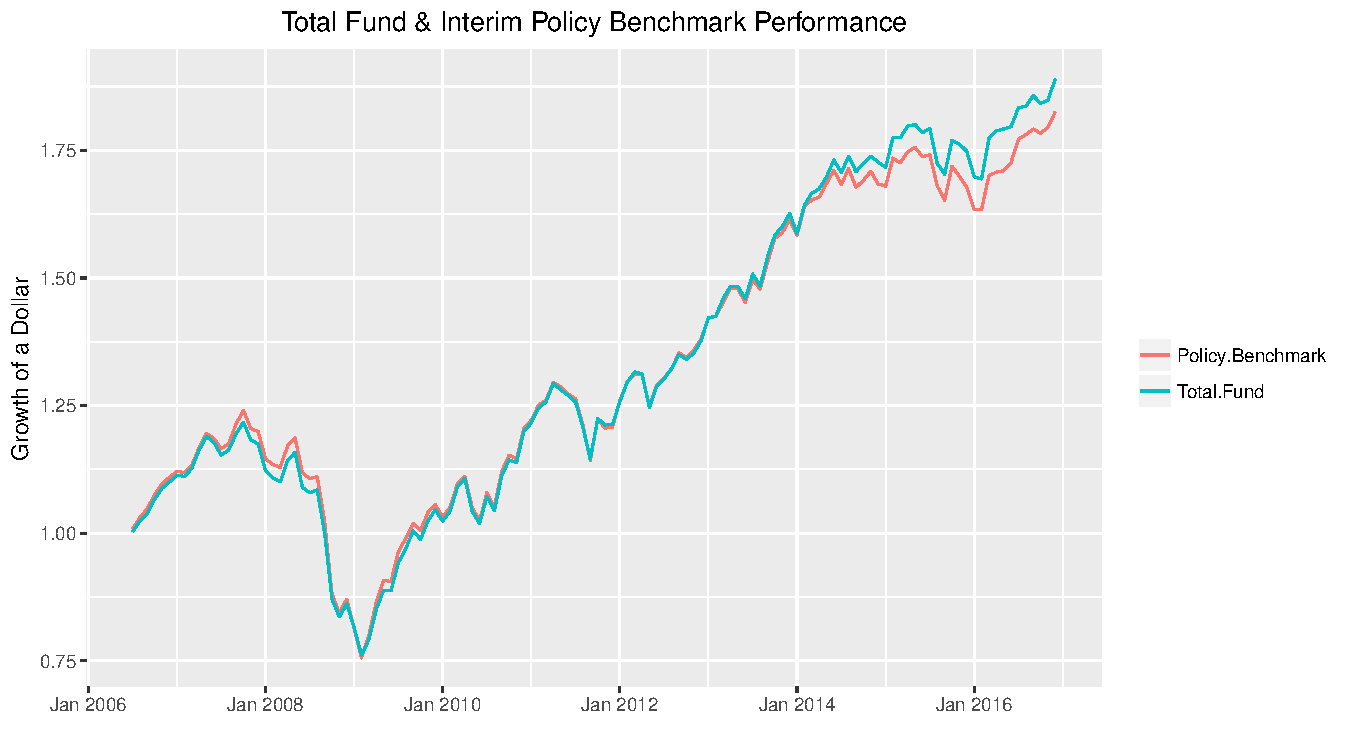
\includegraphics[width=\maxwidth]{figure/total_return-1} 

\end{knitrout}
\end{frame}
%
\begin{frame}[fragile]{Total Fund Excess Return Decomposition}

\begin{knitrout}
\definecolor{shadecolor}{rgb}{0.969, 0.969, 0.969}\color{fgcolor}
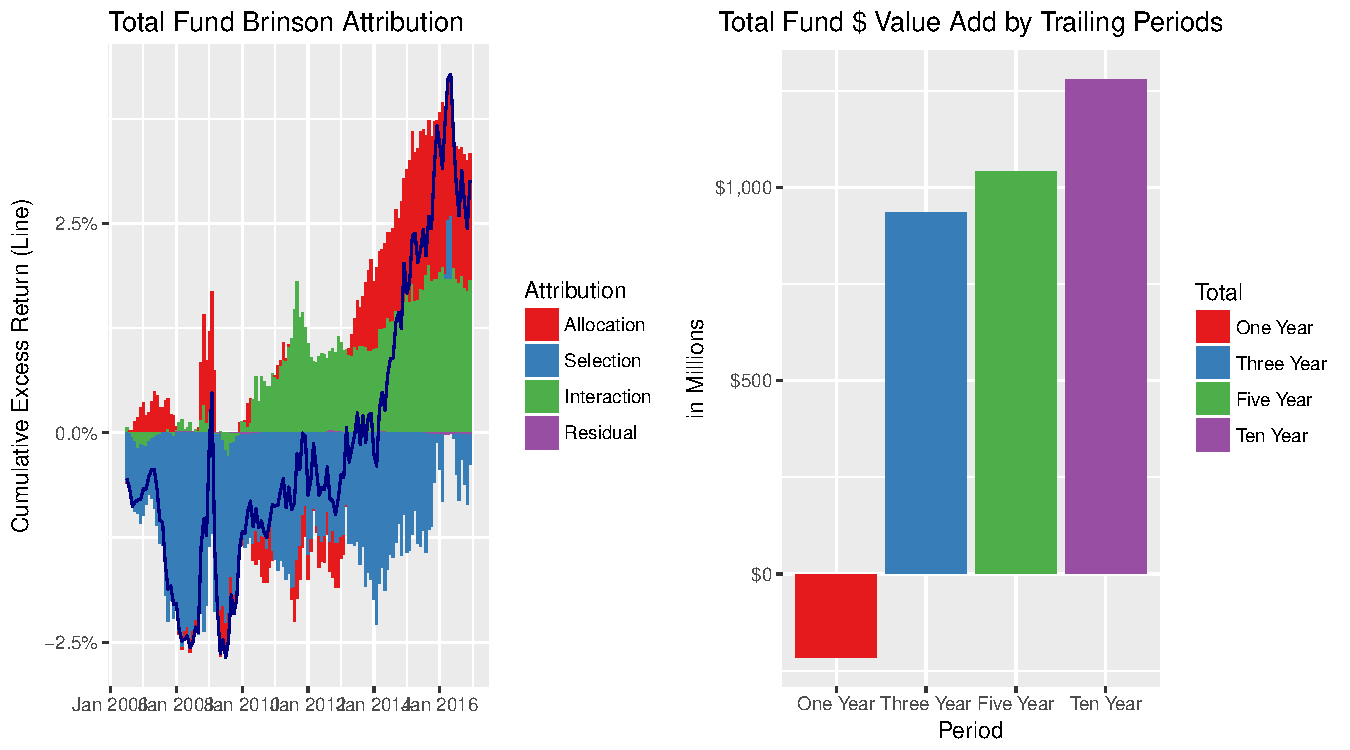
\includegraphics[width=\maxwidth]{figure/tf_brinson-1} 

\end{knitrout}
\end{frame}
%
\begin{frame}[fragile]{Allocation \& Selection Effect Only}

\begin{knitrout}
\definecolor{shadecolor}{rgb}{0.969, 0.969, 0.969}\color{fgcolor}
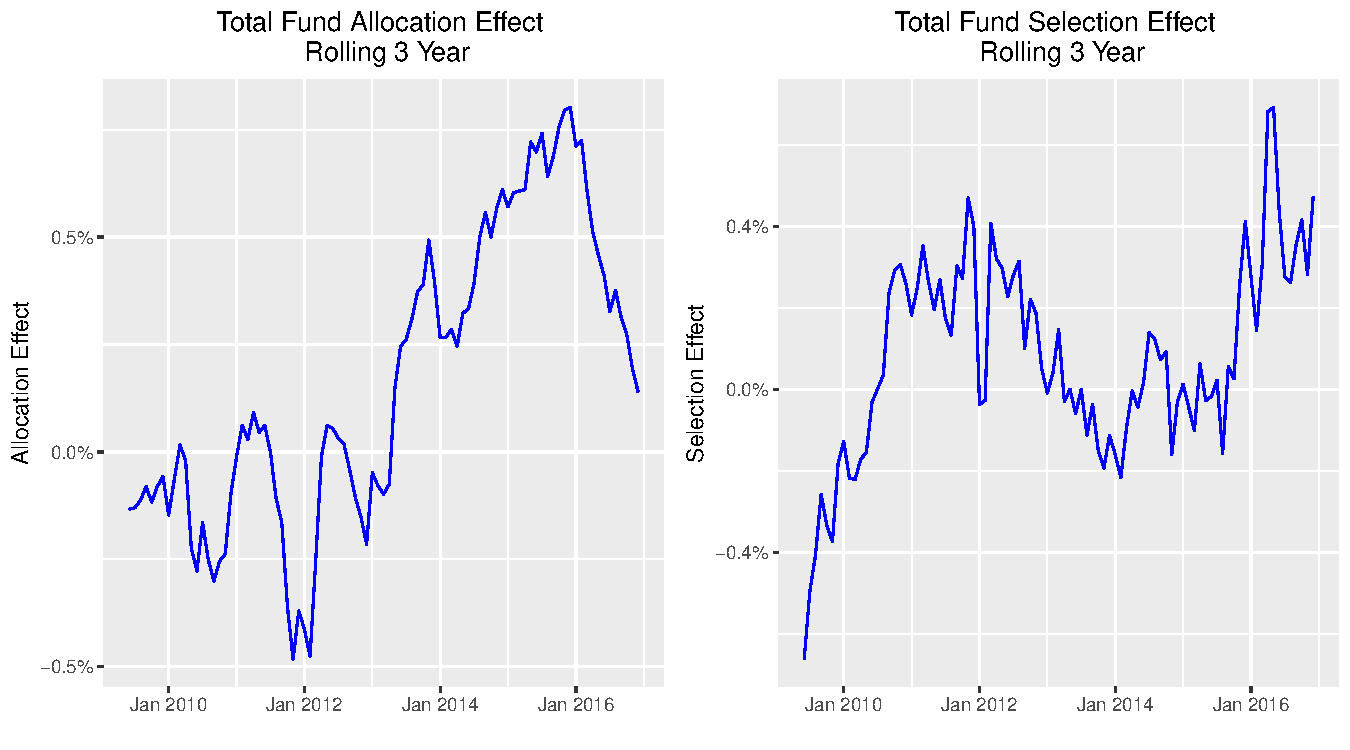
\includegraphics[width=\maxwidth]{figure/tf_breakdown-1} 

\end{knitrout}
\end{frame}
%

\subsubsection{Asset Allocation}
\begin{frame}[fragile]{Historical Strategic Asset Allocation}

The Strategic Asset Allocation is designed to produce steady returns
over a long period of time and is typically completed once every 3
years

\begin{knitrout}
\definecolor{shadecolor}{rgb}{0.969, 0.969, 0.969}\color{fgcolor}
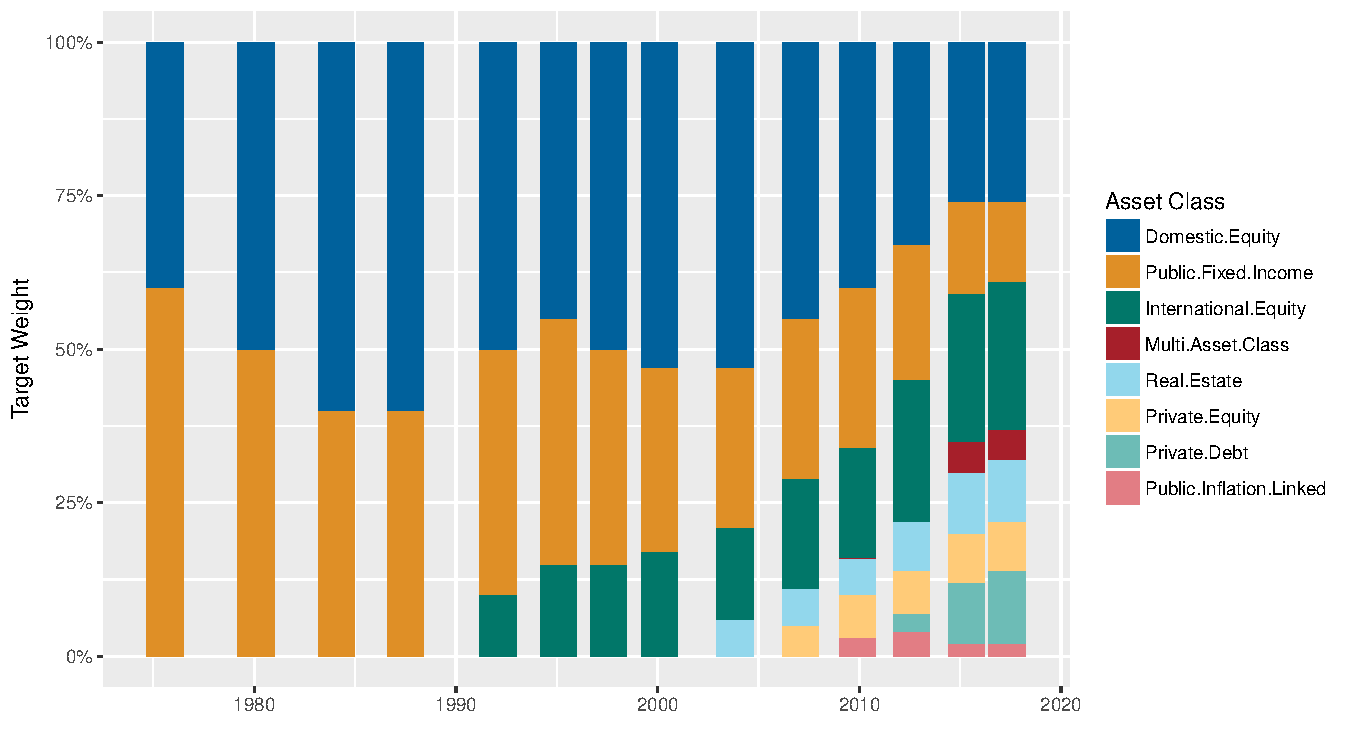
\includegraphics[width=\maxwidth]{figure/saa-1} 

\end{knitrout}
\end{frame}
%
\begin{frame}[fragile]{Allocation and Active Weights}

\begin{knitrout}
\definecolor{shadecolor}{rgb}{0.969, 0.969, 0.969}\color{fgcolor}
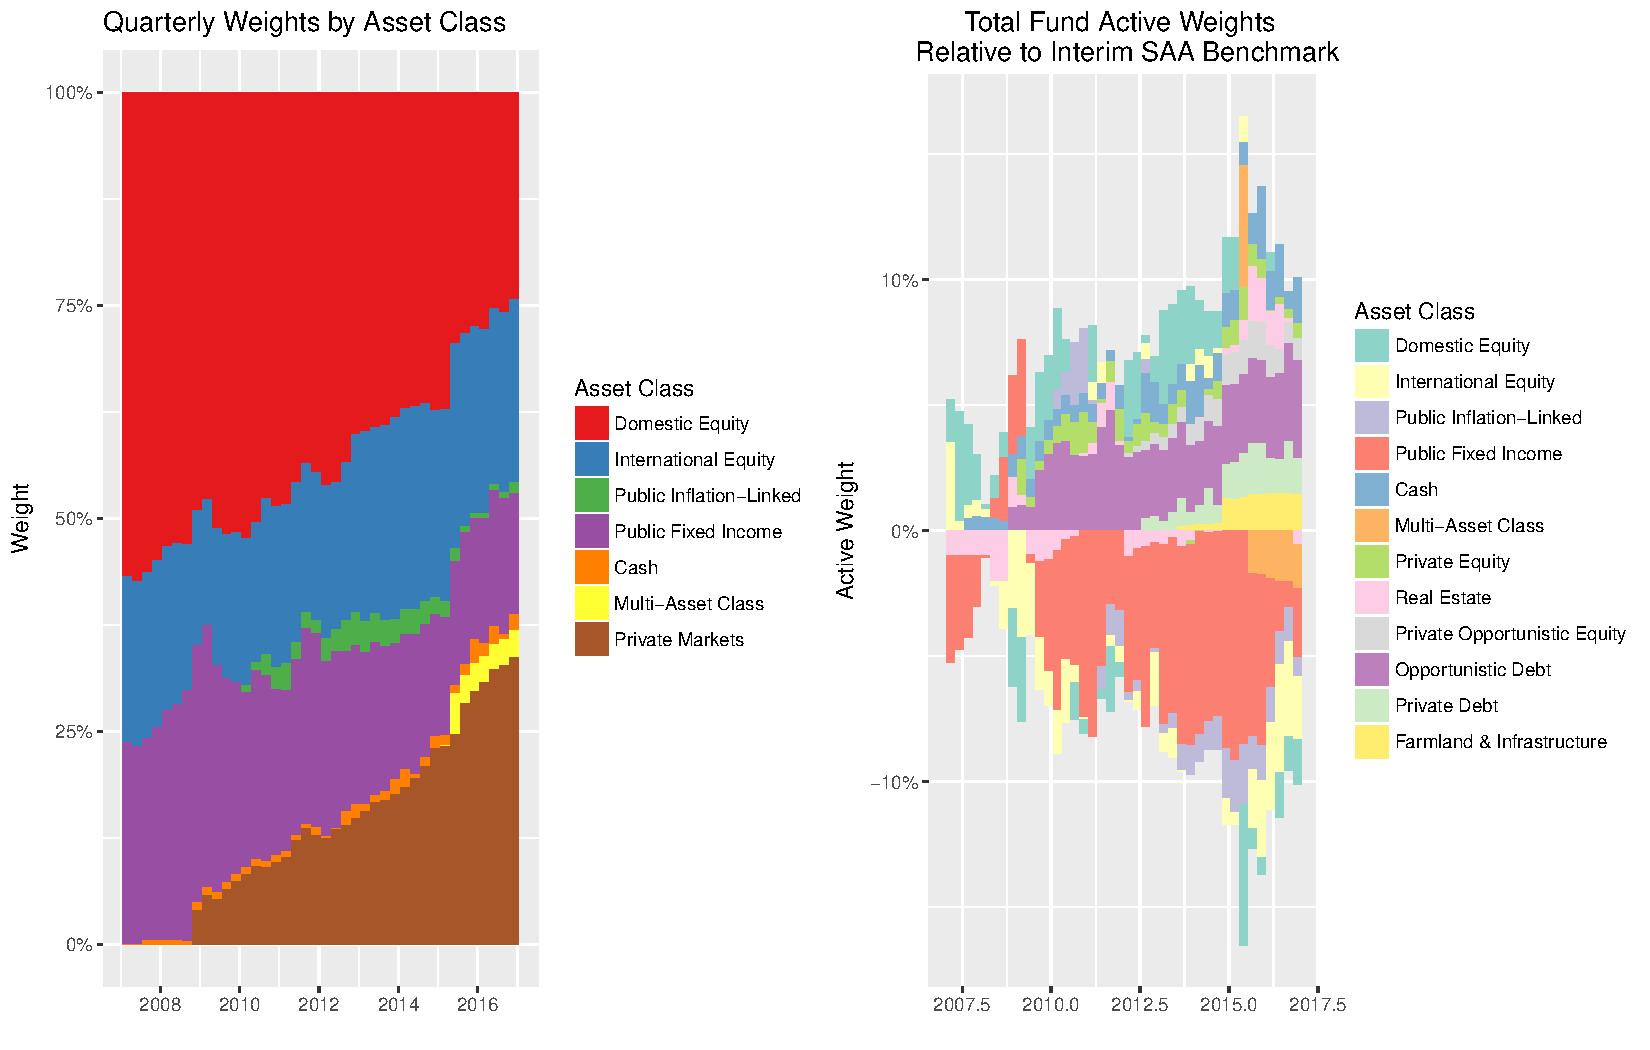
\includegraphics[width=\maxwidth]{figure/tf_weights-1} 

\end{knitrout}
\end{frame}
%

\subsubsection{Equities}
\begin{frame}[fragile]{Public Equity Performance Summary}

\begin{knitrout}
\definecolor{shadecolor}{rgb}{0.969, 0.969, 0.969}\color{fgcolor}
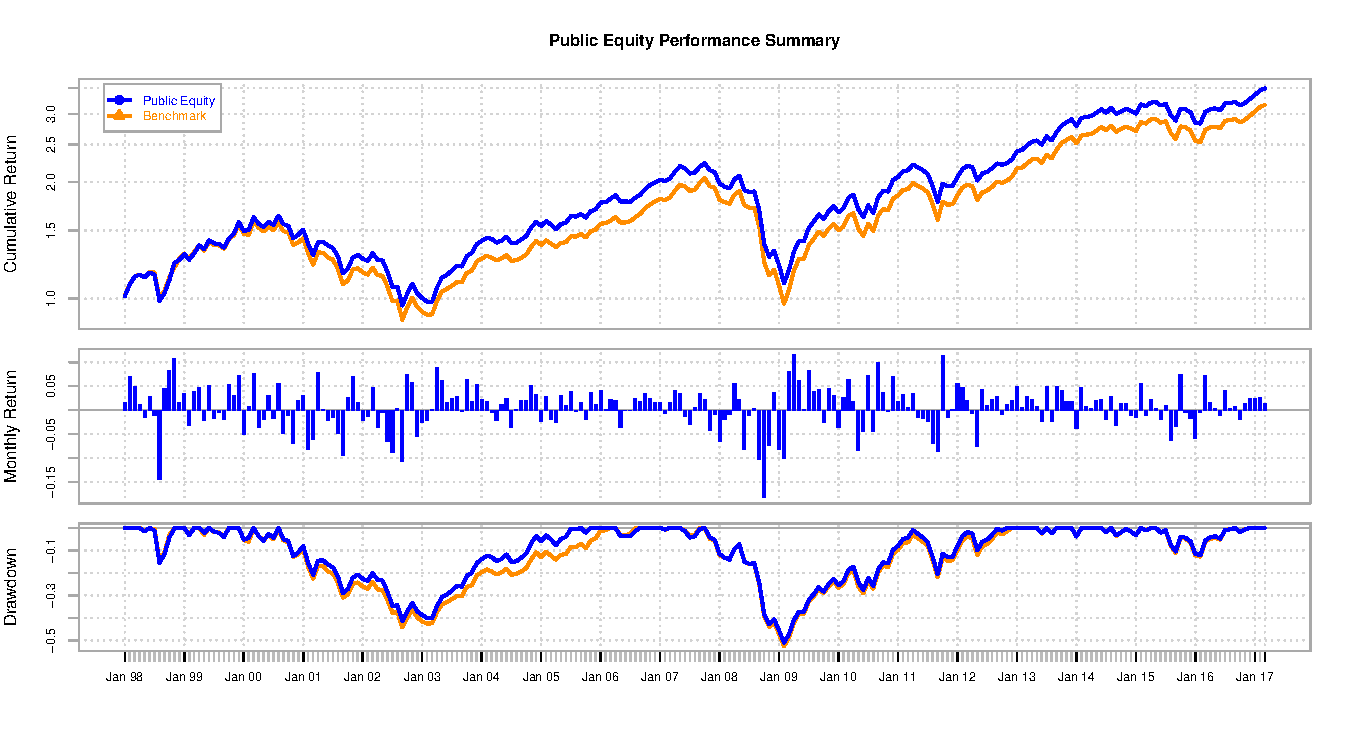
\includegraphics[width=\maxwidth]{figure/equities-1} 

\end{knitrout}
\end{frame}
%
\begin{frame}[fragile]{Public Equity Brinson Attribution}

\begin{knitrout}
\definecolor{shadecolor}{rgb}{0.969, 0.969, 0.969}\color{fgcolor}
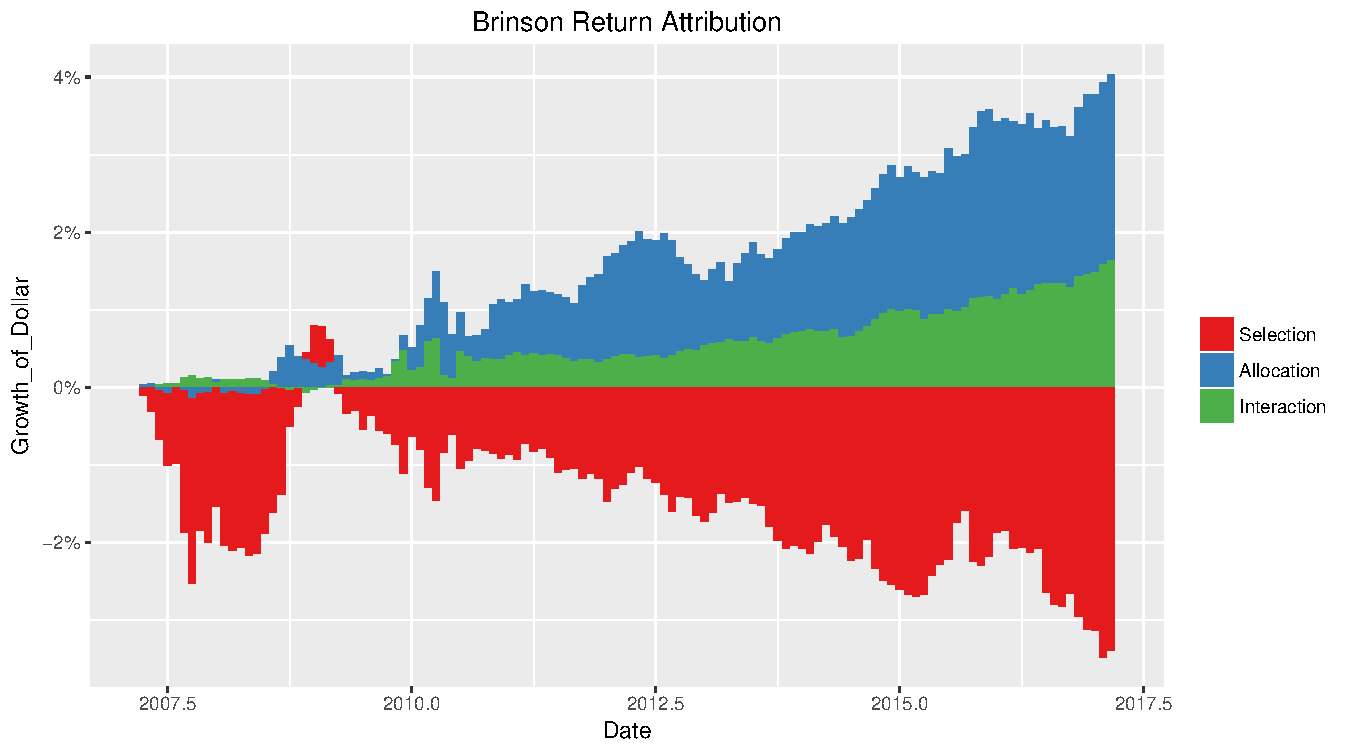
\includegraphics[width=\maxwidth]{figure/eq_attribution-1} 

\end{knitrout}
\end{frame}
%
\begin{frame}[fragile]{Allocation \& Selection Effect Only}

\begin{knitrout}
\definecolor{shadecolor}{rgb}{0.969, 0.969, 0.969}\color{fgcolor}
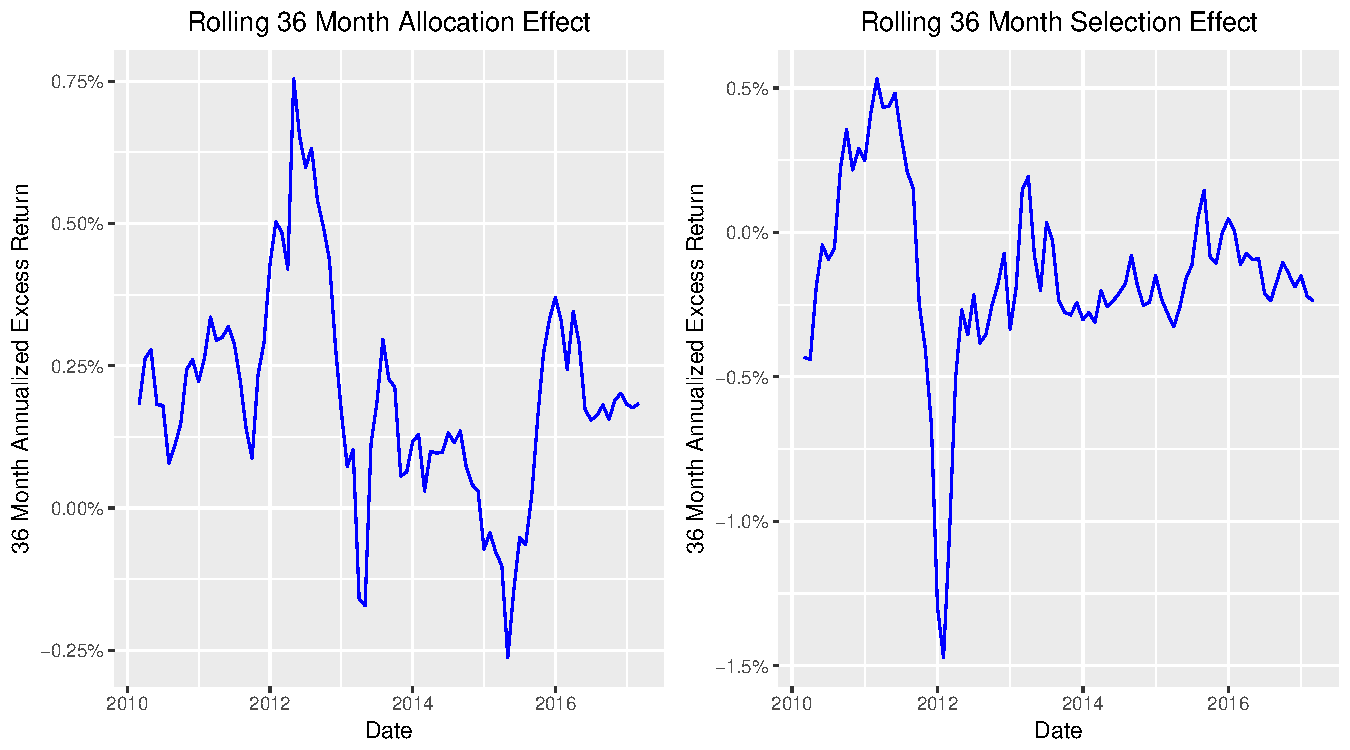
\includegraphics[width=\maxwidth]{figure/eq_rolling-1} 

\end{knitrout}
\end{frame}
%
\begin{frame}[fragile]{Recent E Portfolio Strategy Enhancements }

\begin{knitrout}
\definecolor{shadecolor}{rgb}{0.969, 0.969, 0.969}\color{fgcolor}
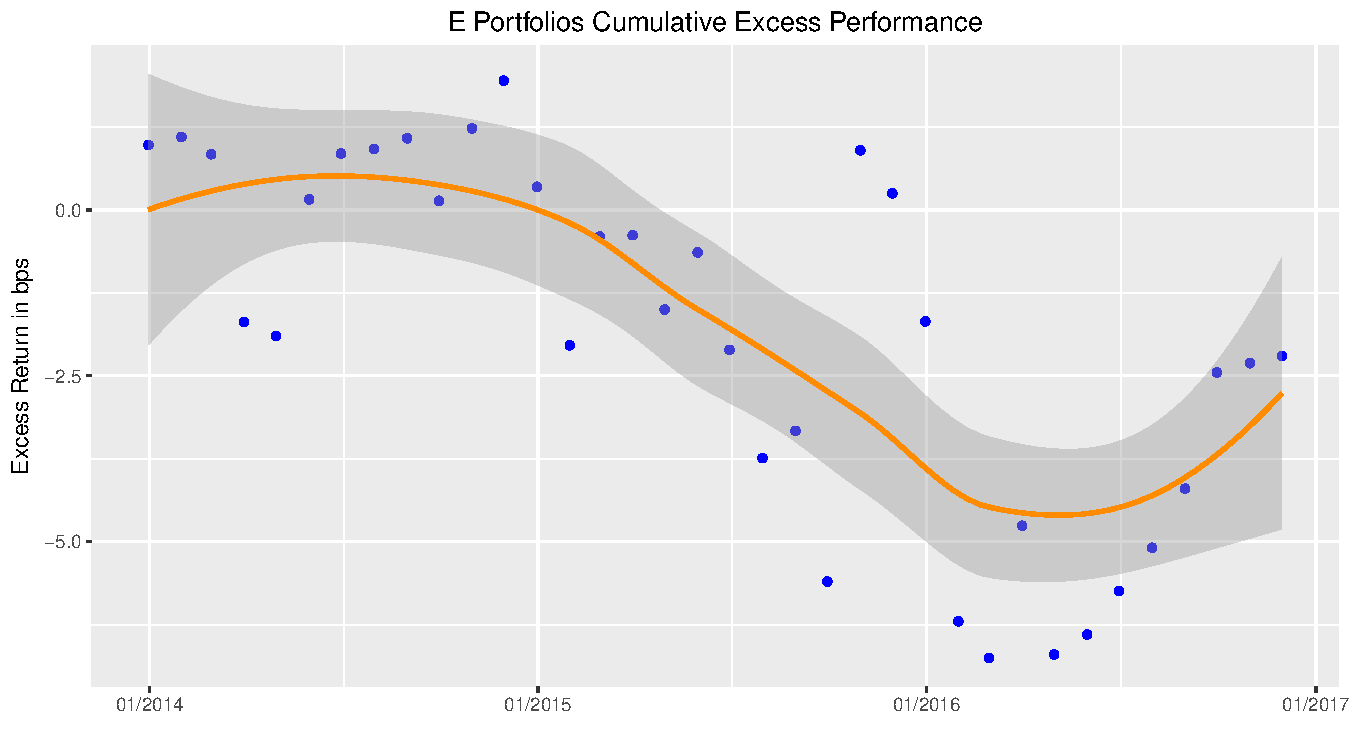
\includegraphics[width=\maxwidth]{figure/e_portfolios-1} 

\end{knitrout}
\end{frame}
%
\begin{frame}[fragile]{Private \& Opportunistic Equity}

\begin{knitrout}
\definecolor{shadecolor}{rgb}{0.969, 0.969, 0.969}\color{fgcolor}
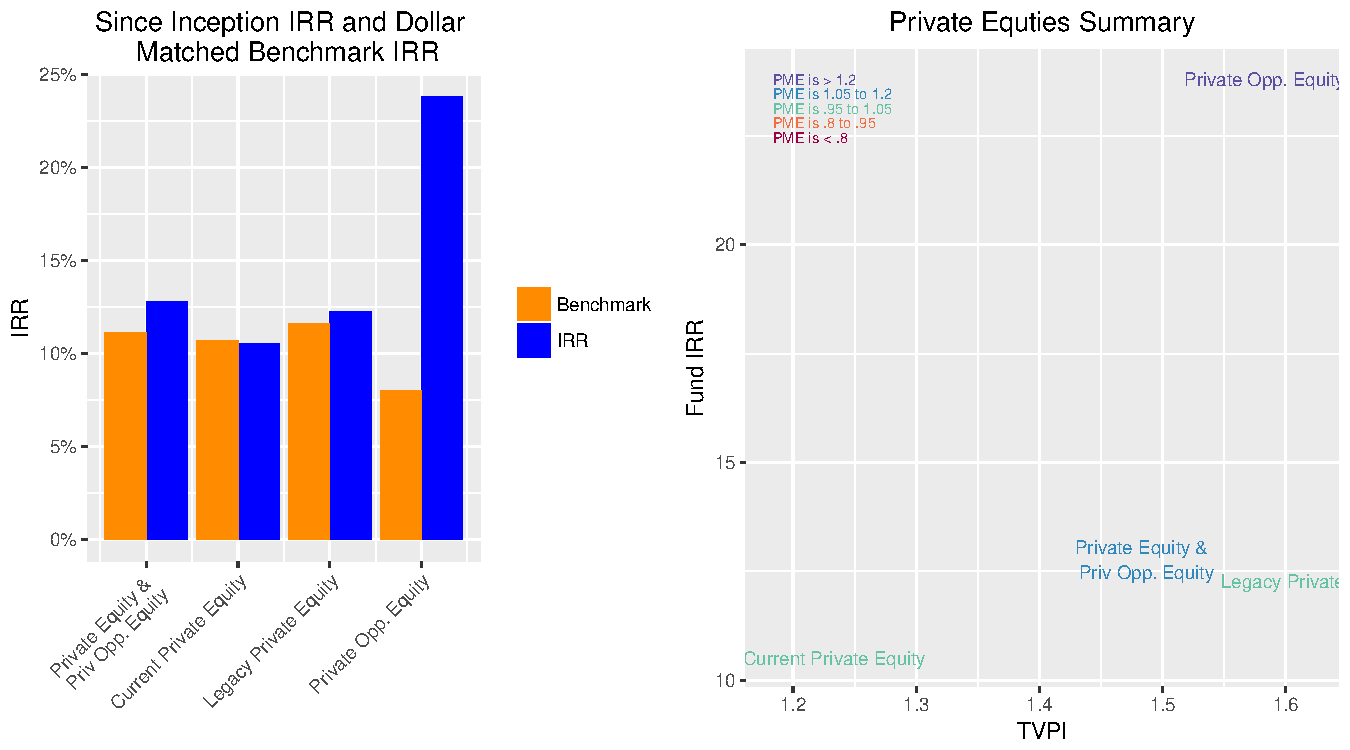
\includegraphics[width=\maxwidth]{figure/eq_privates-1} 

\end{knitrout}
\end{frame}
%

\subsubsection{Fixed Income}
\begin{frame}[fragile]{Public Fixed Income Performance Summary}

\begin{knitrout}
\definecolor{shadecolor}{rgb}{0.969, 0.969, 0.969}\color{fgcolor}
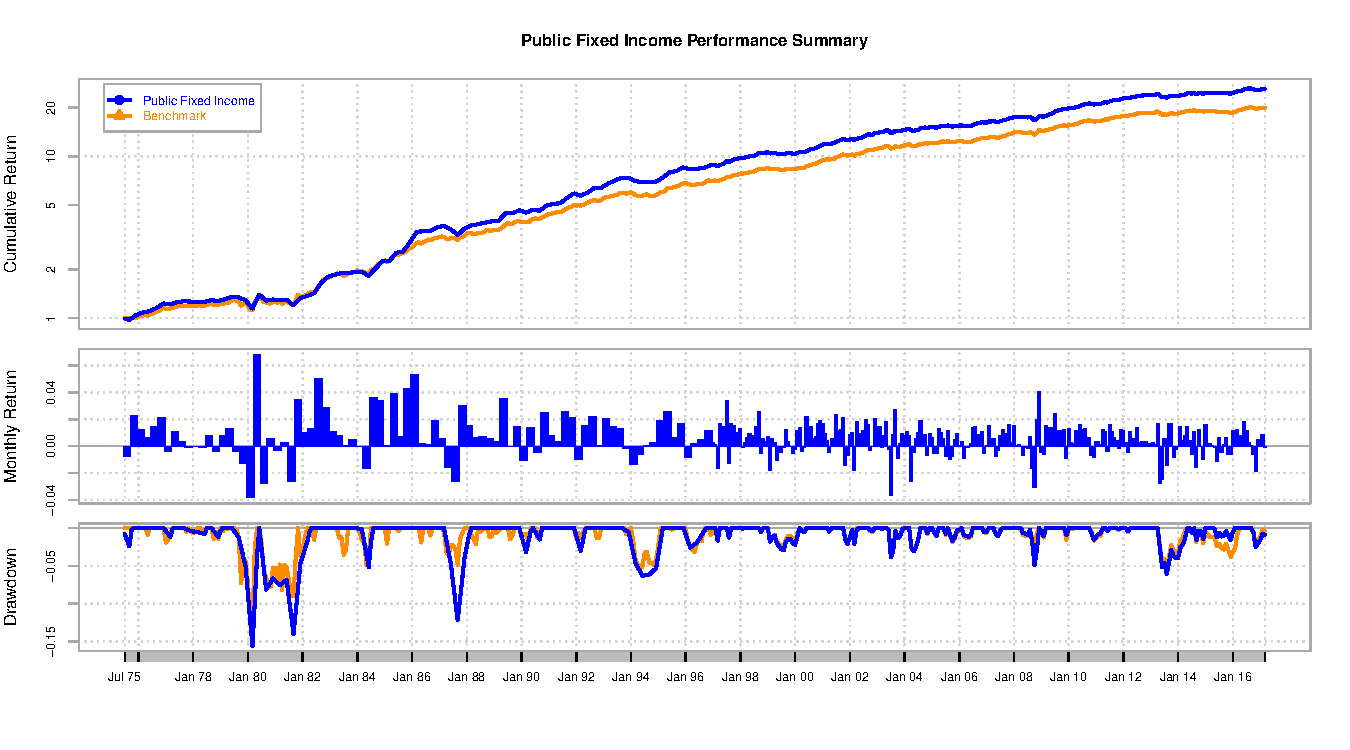
\includegraphics[width=\maxwidth]{figure/fi_summary-1} 

\end{knitrout}
\end{frame}
%
\begin{frame}[fragile]{Public Fixed Income Brinson Attribution}

\begin{knitrout}
\definecolor{shadecolor}{rgb}{0.969, 0.969, 0.969}\color{fgcolor}
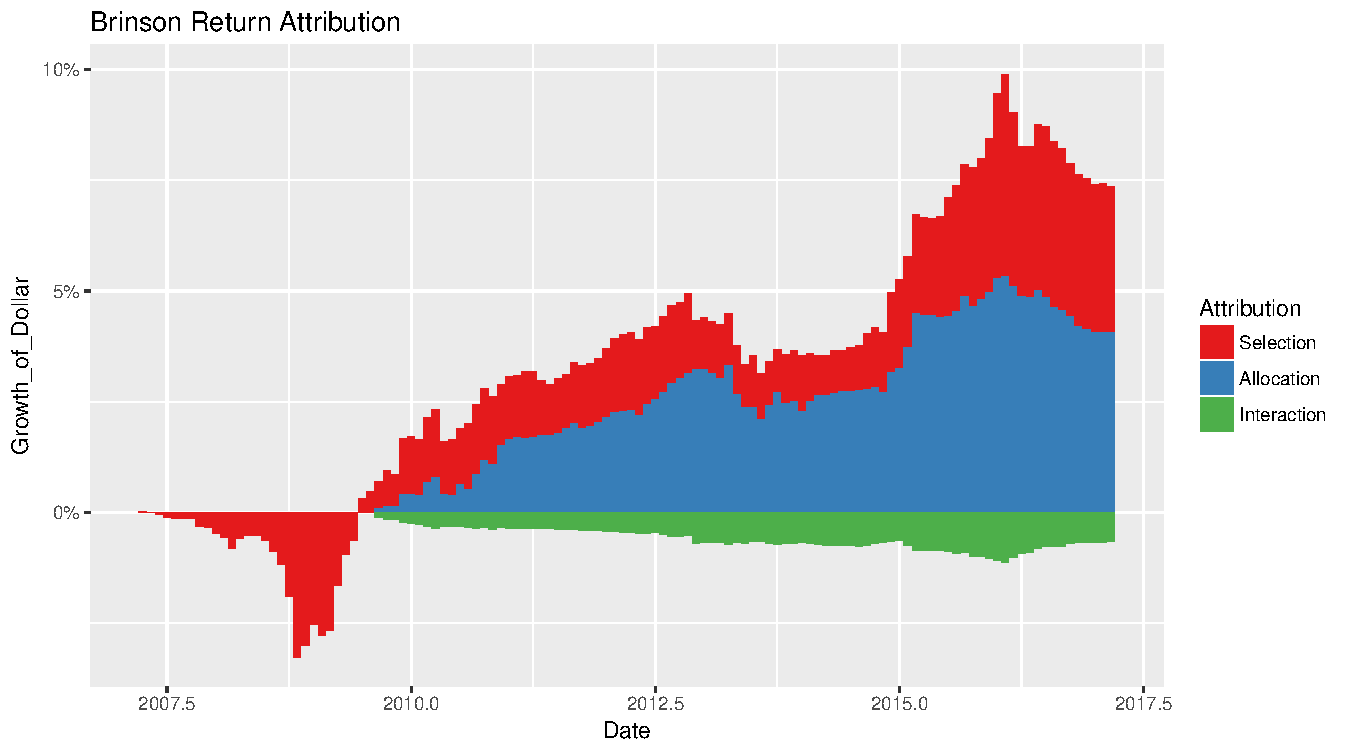
\includegraphics[width=\maxwidth]{figure/fi_attribution-1} 

\end{knitrout}
\end{frame}
%
\begin{frame}[fragile]{Allocation \& Selection Effect Only}

\begin{knitrout}
\definecolor{shadecolor}{rgb}{0.969, 0.969, 0.969}\color{fgcolor}
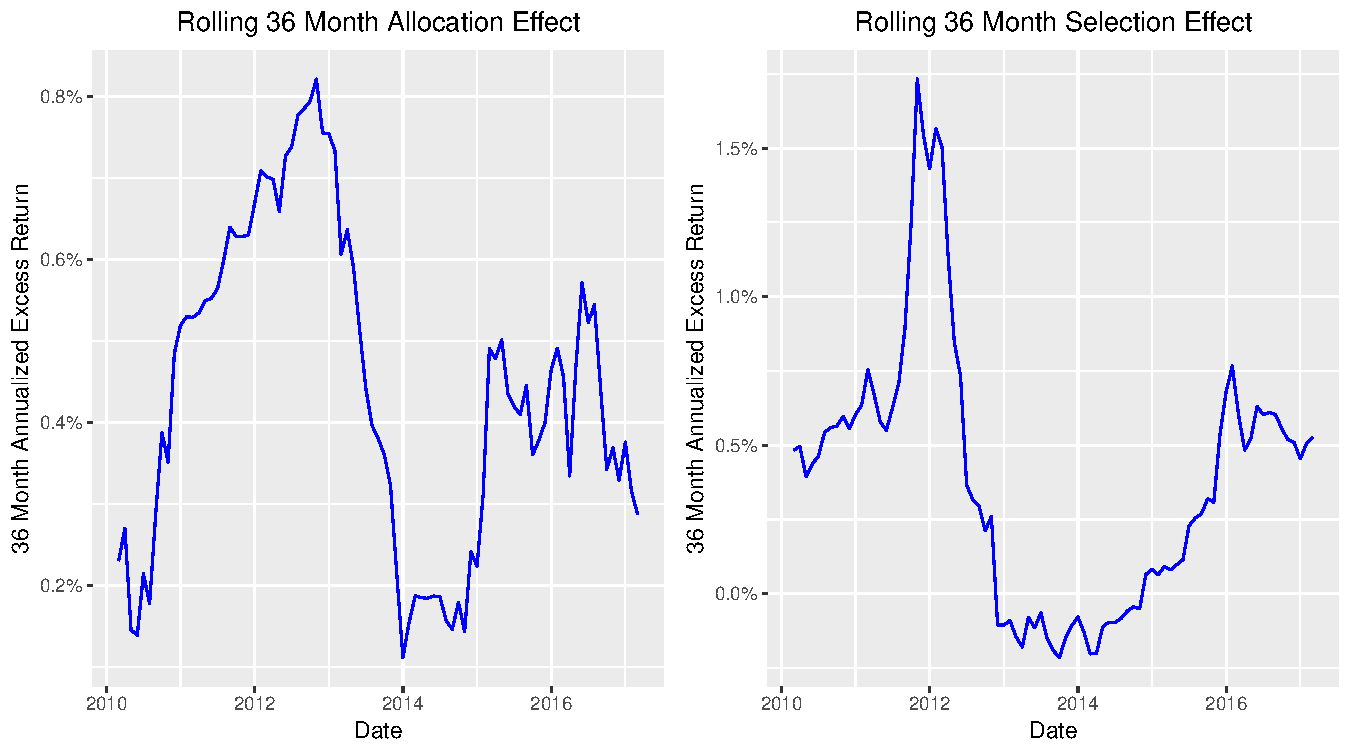
\includegraphics[width=\maxwidth]{figure/fi_rolling-1} 

\end{knitrout}
\end{frame}
%
\begin{frame}[fragile]{Private \& Opportunistic Debt Summary}

\begin{knitrout}
\definecolor{shadecolor}{rgb}{0.969, 0.969, 0.969}\color{fgcolor}
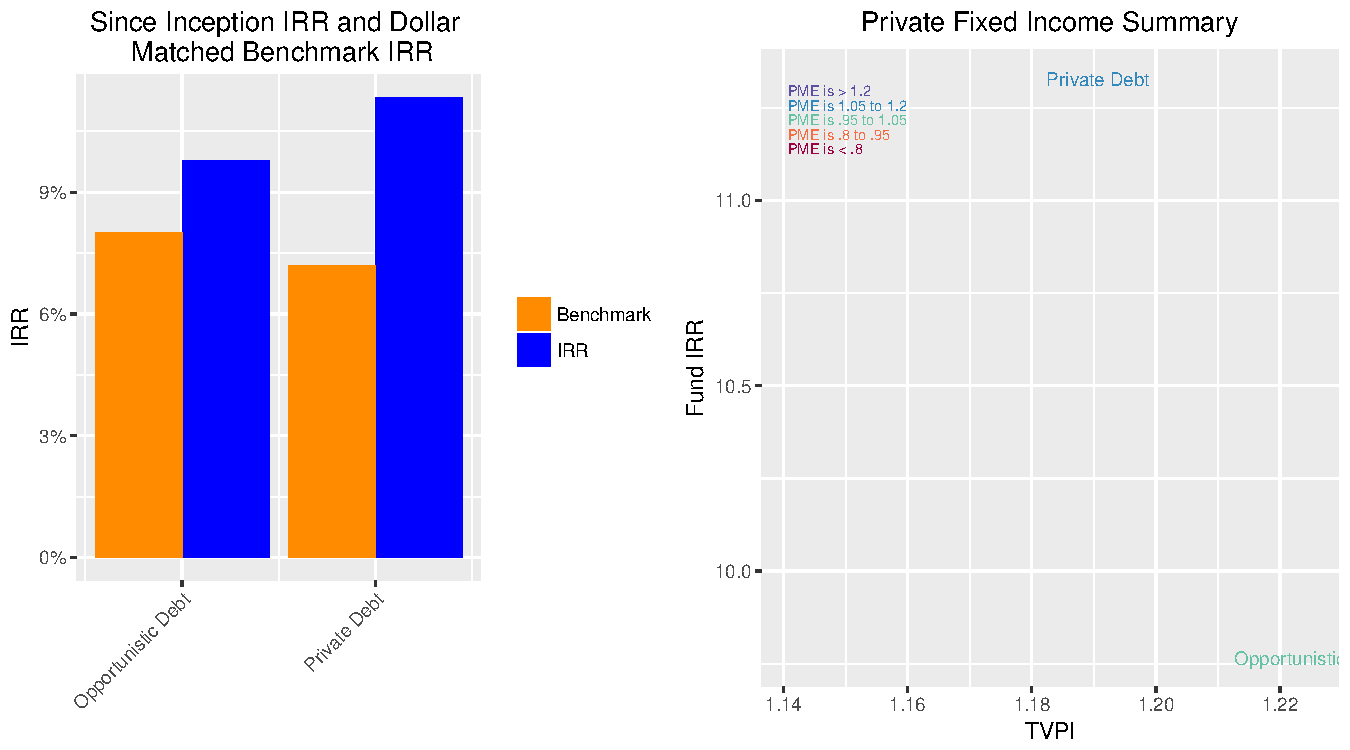
\includegraphics[width=\maxwidth]{figure/fi_privates-1} 

\end{knitrout}
\end{frame}
%

\subsubsection{Real Estate}
\begin{frame}[fragile]{Real Estate Summary}

\begin{knitrout}
\definecolor{shadecolor}{rgb}{0.969, 0.969, 0.969}\color{fgcolor}
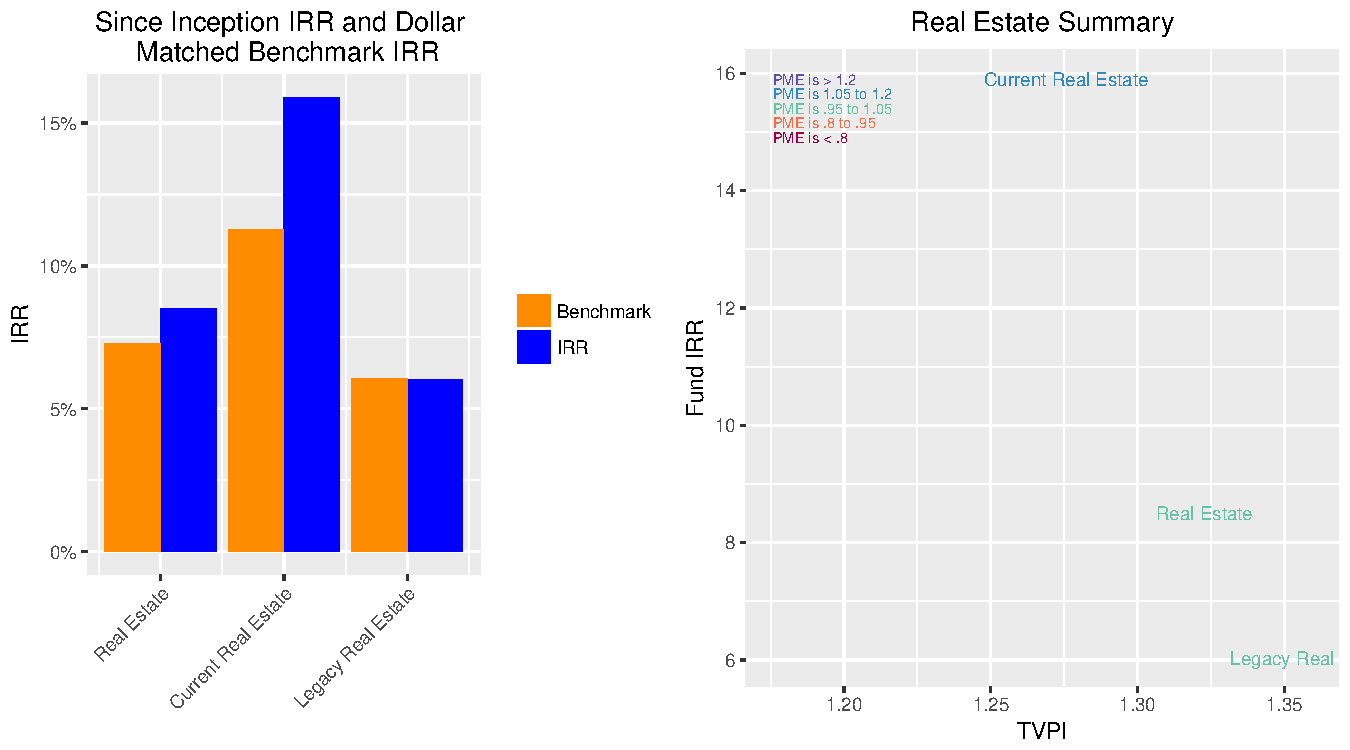
\includegraphics[width=\maxwidth]{figure/real_estate_sum-1} 

\end{knitrout}

\end{document}
\end{frame}
%

\section{Organization}

\subsection{Organization Chart}
\begin{frame}{Organization Chart}

\includegraphics[width=11cm,height=8cm]{3P__IMD_Karl_New_Trustee_Orientation_2017_imd_org_chart_v7.pdf}
\end{frame}
%
\begin{frame}{Project Management}

\includegraphics[width=11cm,height=8cm]{4P__IMD_Karl_R_projects_IMD_Projects_imd_projects.pdf}
\end{frame}
%

\subsection{Key People}
\begin{frame}{Karl Polen, CIO}
\begin{itemize}
\item {\scriptsize{}Associated with ASRS since 1994}{\scriptsize \par}
\begin{itemize}
\item {\scriptsize{}Board member 1994 to 2007 including multiple terms as
chairman of the board and chair of investments}{\scriptsize \par}
\item {\scriptsize{}Head of Private Markets Investing 2010 to 2016}{\scriptsize \par}
\item {\scriptsize{}CIO since 2016}{\scriptsize \par}
\end{itemize}
\item {\scriptsize{}Experience prior to ASRS}{\scriptsize \par}
\begin{itemize}
\item {\scriptsize{}33 years private sector experience}{\scriptsize \par}
\begin{itemize}
\item {\scriptsize{}Bulk of experience in CFO and COO roles for two major
real estate operators based in Phoenix}{\scriptsize \par}
\item {\scriptsize{}Extensive deal experience negotiating a wide range of
transactions involving billions of value}{\scriptsize \par}
\item {\scriptsize{}Operational experience supervising teams of over 1,000
people in diverse business activities}{\scriptsize \par}
\end{itemize}
\item {\scriptsize{}Board and other Memberships}{\scriptsize \par}
\begin{itemize}
\item {\scriptsize{}Central Arizona Project \textendash{} board member 1996
to 2000}{\scriptsize \par}
\item {\scriptsize{}Boys and Girls Clubs of Metropolitan Phoenix \textendash{}
board member 2005 to 2010}{\scriptsize \par}
\item {\scriptsize{}National Academy of Recording Arts and Sciences \textendash{}
voting member since 1977 }{\scriptsize \par}
\end{itemize}
\end{itemize}
\item {\scriptsize{}Education }{\scriptsize \par}
\begin{itemize}
\item {\scriptsize{}Vanderbilt University, Master of Business Administration
(graduated tied for first in class)}{\scriptsize \par}
\item {\scriptsize{}Certified Public Accountant (highest score in state
on CPA exam, license currently inactive)}{\scriptsize \par}
\item {\scriptsize{}University of Tennessee, studies in mathematics and
computer science}{\scriptsize \par}
\item {\scriptsize{}University of Illinois, Bachelor of Music}{\scriptsize \par}
\end{itemize}
\end{itemize}
\end{frame}
%
\begin{frame}{Al Alaimo, Sr Portfolio Manager (fixed income, cash, liquid alternatives)}
\begin{itemize}
\item {\scriptsize{}Senior Fixed Income Portfolio Manager}{\scriptsize \par}
\item {\scriptsize{}Joined ASRS in 2009 }{\scriptsize \par}
\item {\scriptsize{}Previously. Portfolio Manager and Director of Research
for Seneca Capital Management LLC in San Francisco and a Managing
Director in high yield bond research for Banc of America Securities
LLC in New York. }{\scriptsize \par}
\item {\scriptsize{}MBA in Finance from the University of Rochester and
a BS in accounting and finance from Syracuse University}{\scriptsize \par}
\item {\scriptsize{}From 2010-2013, taught an undergraduate course on Fixed
Income which he created for the Finance Department at the W.P. Carey
School of Business at Arizona State University. }{\scriptsize \par}
\item {\scriptsize{}Chartered Financial Analyst (CFA)}{\scriptsize \par}
\item {\scriptsize{}Certified Public Accountant (CPA)}{\scriptsize \par}
\end{itemize}
\end{frame}
%
\begin{frame}{Eric Glass, Sr Portfolio Manager (equities and real estate)}
\begin{itemize}
\item {\scriptsize{}Joined ASRS in 2008}{\scriptsize \par}
\begin{itemize}
\item {\scriptsize{}Analyst across multiple asset classes 2008 to 2013}{\scriptsize \par}
\item {\scriptsize{}Private Markets investing 2013 to 2016}{\scriptsize \par}
\item {\scriptsize{}Head of Private Markets \& Equities since 2016}{\scriptsize \par}
\end{itemize}
\item {\scriptsize{}Experience prior to ASRS}{\scriptsize \par}
\begin{itemize}
\item {\scriptsize{}7 years private sector experience}{\scriptsize \par}
\begin{itemize}
\item {\scriptsize{}Majority of experience as equity analyst; fundamental
analysis and forensic accounting}{\scriptsize \par}
\item {\scriptsize{}Experience in tax and advisory for HNW clients in public
accounting}{\scriptsize \par}
\end{itemize}
\item {\scriptsize{}Board and other Memberships}{\scriptsize \par}
\begin{itemize}
\item {\scriptsize{}Junior Achievement volunteer }{\scriptsize \par}
\item {\scriptsize{}Habitat for Humanity volunteer }{\scriptsize \par}
\item {\scriptsize{}Feed My Starving Children volunteer }{\scriptsize \par}
\end{itemize}
\end{itemize}
\item {\scriptsize{}Education }{\scriptsize \par}
\begin{itemize}
\item {\scriptsize{}University of Minnesota, Master of Business Administration}{\scriptsize \par}
\begin{itemize}
\item {\scriptsize{}Finance \& Entrepreneurship}{\scriptsize \par}
\end{itemize}
\item {\scriptsize{}Iowa State University, Bachelor of Science with Honors
\& Distinction}{\scriptsize \par}
\begin{itemize}
\item {\scriptsize{}Finance \& Accounting; Economics}{\scriptsize \par}
\end{itemize}
\item {\scriptsize{}Chartered Financial Analyst (CFA)}{\scriptsize \par}
\item {\scriptsize{}Certified Public Accountant (CPA) (license currently
inactive)}{\scriptsize \par}
\item {\scriptsize{}Chartered Alternative Investment Analyst (CAIA)}{\scriptsize \par}
\end{itemize}
\end{itemize}
\end{frame}
%
\begin{frame}{Kerry White, Assistant CIO (operations, compliance and reporting)}
\begin{itemize}
\item {\scriptsize{}Joined ASRS since 2011}{\scriptsize \par}
\begin{itemize}
\item {\scriptsize{}Private Markets Asset Manager 2011 to 2016}{\scriptsize \par}
\item {\scriptsize{}Assistant CIO since 2016}{\scriptsize \par}
\end{itemize}
\item {\scriptsize{}Experience prior to ASRS}{\scriptsize \par}
\begin{itemize}
\item {\scriptsize{}24 years of private sector experience}{\scriptsize \par}
\begin{itemize}
\item {\scriptsize{}20 years of experience in public accounting, practice
areas include auditing, management consulting, training and tax}{\scriptsize \par}
\item {\scriptsize{}COO and CFO experience for non-profit and manufacturing
industries}{\scriptsize \par}
\item {\scriptsize{}Operational expertise, internal control, network and
system administration for variety of clients and employers}{\scriptsize \par}
\end{itemize}
\item {\scriptsize{}Board and other Memberships}{\scriptsize \par}
\begin{itemize}
\item {\scriptsize{}Arizona Bicycle Club \textendash{} president 2015 to
current, board member 2013 to 2015, 300+ member organization}{\scriptsize \par}
\item {\scriptsize{}Maricopa County Parks Community Park Volunteer, Usury
Park 2010 - 2015 }{\scriptsize \par}
\item {\scriptsize{}AICPA \textendash{} member 1997 to current, AZCPA \textendash{}
member 2010 to current}{\scriptsize \par}
\end{itemize}
\end{itemize}
\item {\scriptsize{}Education }{\scriptsize \par}
\begin{itemize}
\item {\scriptsize{}Grand Canyon University, MBA with an Emphasis in Finance
(3.97 GPA)}{\scriptsize \par}
\item {\scriptsize{}Certified Public Accountant (Active license in both
Arizona and Washington State)}{\scriptsize \par}
\item {\scriptsize{}Specialty Certifications in Governmental and Non-Profit
Accounting \& Auditing, and Technology}{\scriptsize \par}
\item {\scriptsize{}St. Martins University, Bachelor of Arts in Accounting,
Cum Laude}{\scriptsize \par}
\end{itemize}
\end{itemize}
\end{frame}
%

\subsection{Technology}
\begin{frame}{IMD is Committed to State of the Art Technology}
\begin{itemize}
\item IMD is invests effort and resources to technology in part because
\begin{itemize}
\item Automation of repetitive tasks improves quality and saves money
\item Implementation of graphical reporting methods improves communication
and makes it more impactful
\end{itemize}
\item More importantly, technology helps us make money 
\begin{itemize}
\item by implementing state of the art performance measurement techniques
which provide feedback and identify areas for improvement
\item by allowing us to implement the most sophisticated statistical and
modeling methods not practical any other way
\item these methods help identify and test trading and investment methodologies
and strategies
\end{itemize}
\item ASRS has been a leader in the adoption of these sophisticated methods
\begin{itemize}
\item Several members of the team have expertise as ``coders'' enabling
us to efficiently implement new methods
\item By way of example, ASRS implemented ``PME'' methods for performance
evaluation as they were identified in academic literature and years
before they were commercially available
\end{itemize}
\end{itemize}
\cleardoublepage{}
\end{frame}
%

\section{Policies, Governance and Compliance}

\subsection{Investment Policy Statement}
\begin{frame}{Investment Policy Statement - Purpose}
\begin{itemize}
\item The Investment Policy Statement (\href{https://www.azasrs.gov/sites/default/files/pdf/Investment\%20Policy\%20Statement\%20-\%20may\%202015_0.pdf}{Link to IPS})
is designed to communicate and establish the following:
\begin{itemize}
\item investment beliefs,
\item goals \& objectives,
\item constraints, and
\item guidelines for development and implementation of the ASRS strategic
and tactical asset allocation policy.
\end{itemize}
\item The investment policy statement is important to the long term success
of the ASRS investment objectives.
\item The investment policy statement was developed with the following goals:
\begin{itemize}
\item Clearly and explicity establish the parameters governing ASRS assets
\item Establish a target asset allocation that is both long-term and dynamic
to take advantage of market opportunities and expected to achieve
its investment rate of return objectives
\item Protect the financial health of the ASRS
\item Establish a framework for monitoring investment activity and facilitate
communication between Board, Staff and other involved parties.
\end{itemize}
\end{itemize}
\end{frame}
%
\begin{frame}{Investment Policy Statement - Goals}
\begin{itemize}
\item {\small{}These are macro-level expected outcomes that the ASRS wants
to achieve through its investment program.}{\small \par}
\item {\small{}Goals}:
\begin{itemize}
\item {\footnotesize{}Maximizes fund rates of return for acceptable levels
of fund risk.}{\footnotesize \par}
\item {\footnotesize{}Achieves 75th percentile rates of return compared
to peers.}{\footnotesize \par}
\item {\footnotesize{}Achieves long-term fund rates of return equal to or
greater than the actuarial assumed interest rate.}{\footnotesize \par}
\item {\footnotesize{}Achieves long-term econcomic and actuarial funded
states of 100 percent}{\footnotesize \par}
\item {\footnotesize{}Mitigates contribution rate volatility}{\footnotesize \par}
\end{itemize}
\item {\small{}Collectively, the above goals incorporate the following elemets
that are important for a fund's comprehensive investment structure:}{\small \par}
\begin{itemize}
\item {\footnotesize{}Complementary use of absolute and relative rates-of-return
perspectives.}{\footnotesize \par}
\item {\footnotesize{}Complementary use of asset-only and asset-liability
perspectives.}{\footnotesize \par}
\item {\footnotesize{}Complementary use of economic and actuarial perspectives.}{\footnotesize \par}
\end{itemize}
\end{itemize}
\end{frame}
%
\begin{frame}{Investment Policy Statement - Objectives}
\begin{itemize}
\item {\small{}Objectives:}{\small \par}
\begin{itemize}
\item {\footnotesize{}Acheive a 20-year rolling annual total fund net rate
of return equal to or greater than the actuarial assumed interest
rate of 8\%.}{\footnotesize \par}
\item {\footnotesize{}Acheive 1-year and 3-year rolling acutal total fund
net rates of return equal to or grather than the return of the ASRS
asset allocation policy (SAAP) benchmark.}{\footnotesize \par}
\item {\footnotesize{}Acheive 1-year and 3-year rolling annual net rates
of return for ASRS strategic asset claases that are equal to or greater
than their respective strategic asset class benchmarks.}{\footnotesize \par}
\item {\footnotesize{}Ensure sufficient monies are available to meet pension
benefits, health insurance, member refunds, administrative payments,
and other cash-flow requirements.}{\footnotesize \par}
\end{itemize}
\end{itemize}
\end{frame}
%
\begin{frame}{Investment Policy Statement - Investment Beliefs}
\begin{itemize}
\item {\small{}The investment belief are to ensure the developmentof congruent
and synergistic investment strategies, and to ensure the effective
and efficient allocation of resources. They determine the general
paradigm within which investment strategies are developed, investment
ideas are reviewed, and investment decisions are implemented. Modifications
to these beliefs will occur if experiential, academic, conceptiual
and/or practical perspectives suggest that a superior belief system
exists.}{\small \par}
\item {\small{}Asset class decisions are key:}{\small \par}
\begin{itemize}
\item {\footnotesize{}Decisions with respect to which asset classes and
sub-asset classes to invest in and allocations to these have a greater
impact on total fund investment returns than decisions in which specific
securities to invest.}{\footnotesize \par}
\end{itemize}
\item {\small{}Theories and concepts must be sound:}{\small \par}
\begin{itemize}
\item {\footnotesize{}Over longer periods of time, investment outcomes conform
to logical theories and concepts. Significant deviations from theoretically
and conceptually sound investment constructs are usually not sustainable
and typically self-reverting.}{\footnotesize \par}
\end{itemize}
\item {\small{}House capital market views are imperative:}{\small \par}
\begin{itemize}
\item {\footnotesize{}Development and articulation of sound House Views
will ensure consistentcy amount investment decisions, clairy of investment
direction, baselines for debates, and conformity of understanding.}{\footnotesize \par}
\end{itemize}
\end{itemize}
\end{frame}
%
\begin{frame}{Investment Policy Statement - Investment Beliefs (Continued)}
\begin{itemize}
\item {\small{}Investment strategies must be forward looking:}{\small \par}
\begin{itemize}
\item {\footnotesize{}Use forward looking insights, rather than simply relying
on past strategies.}{\footnotesize \par}
\item {\footnotesize{}Public Markets are generally informationally efficient.}{\footnotesize \par}
\end{itemize}
\item {\small{}Market frictions are highly relevant:}{\small \par}
\begin{itemize}
\item {\footnotesize{}And can be significantly deterimental to investment
performance. As a result transactions will initiated only to the extent
there is a strong level of conviction that they will result in increases
investment returns or decreased risks net of all market frictions.}{\footnotesize \par}
\end{itemize}
\item {\small{}Internal investment professionals are the foundation of a
successful investment program.}{\small \par}
\item {\small{}External investment management is beneficial.}{\small \par}
\item {\small{}Investment consultants:}{\small \par}
\begin{itemize}
\item {\footnotesize{}Utilized when there is a need in one of the four areas:
independence, perspective, special skills, and resource allocation.}{\footnotesize \par}
\end{itemize}
\item {\small{}Trustee expertise:}{\small \par}
\begin{itemize}
\item {\footnotesize{}Trustees often have experience in various areas of
investment management and this expertise should be utilized while
ensuring a spearativion between Board oversight and staff man}{\footnotesize \par}
\end{itemize}
\end{itemize}
\end{frame}
%
\begin{frame}{Investment Policy Statement - Investment Considerations}
\begin{itemize}
\item Arizona State Statutes
\begin{itemize}
\item ASRS investments may be limited by Arizona Revised Statues.
\end{itemize}
\item ASRS is managed on a going-concern basis and uses the following timeframes
for construction decisions and contribution rate determinations.
\begin{itemize}
\item Portfolio contruction decisions: Strategic asset allocations focus
on medium term (3 - 5 years) capital market expectations, subject
to the constraint of meeting the long-term assumed actuarial rate
based on long-term (30 year) capital market assumptions. Tactial deviation
decisions are based on shorter-term (less than 3-5 year) captial market
expectations.
\item Contribution rate determination: Liabilities are discounted based
upon long-term capital market expectations. Contribution rates areset
based upon longer (10 year) investment valuation smoothing periods,
and longer-term (30 years 'closed') deficit/surplus amortization periods.
\end{itemize}
\item Liquidity and Cash-Flow
\begin{itemize}
\item Planning for and effectively managing cash to meet anticpated needs
and ensure adequate liquidity.
\end{itemize}
\end{itemize}
\end{frame}
%
\begin{frame}{Investment Policy Statement - Risk Management, Monitoring and Reporting}
\begin{itemize}
\item A risk management framework is applied for identifying, managing and
reporting on ASRS investments.
\item Provide assurance to Executive Management and Board that investment
management programs are designed, implemented and maintained to achieve
investment goals and objectives.
\item Reporting periodicity and detail vary depending on target audience.
\item Use of leverage is determined at the manager level and monitored by
Investment Management and ASRS consultants.
\item Use of derivatives is determined at the manager level and monitored
by Investment Management and ASRS consultants.
\item Management of currency exposure is determined at manager level and
monitored by Investment Management and ASRS consultants.
\end{itemize}
\end{frame}
%
\begin{frame}{Investment Policy Statement - Asset Allocation}
\begin{itemize}
\item The ASRS asset mix will reflect investments in strategic and tactical
asset classes and strategies whose collective risk/return profile
are anticipated to achieve its long-term investment rate of return
goals and objectives.
\item Dynamic approach where initiation and periodicity will primarly be
a function of market dynamics.
\item Study will be used to determin the long-term policy asset weights.
\item Asset reviews in addition to periodic studies are conducted as warrante
or triennally, whichever is shorter.
\item The study may include, but not be limited to the following:
\begin{itemize}
\item Discussion and analysis of existing and evolving asset classes and
investment strategies.
\item Evaluation of expected sources of investment returns, risk and diversification
(quantitatively/ qualitatively). 
\item Reviewing investment industry developments (academic and pragmatic).
\item Utilization of quantitative tools (e.g., efficient frontier mean-variance
optimization, risk budgeting) and evaluation of multiple scenarios. 
\item Reviewing and engaging discussions regarding capital market assumptions. 
\item Reviewing asset allocation policies from other public and non-public
entities.
\end{itemize}
\end{itemize}
\end{frame}
%
\begin{frame}{Investment Policy Statement - Other Topics}
\begin{itemize}
\item The investment policy statement addresses the other following items:
\begin{itemize}
\item Rebalancing
\item Voting of portfolio proxies
\item Securities litigation
\item Securities lending
\item Management of investment fees
\item Roles and responsibilities
\end{itemize}
\cleardoublepage{}
\end{itemize}
\end{frame}
%

\section{Investment Policies}
\begin{frame}{Strategic Investment Policies}
\begin{itemize}
\item Strategic Investment Policies (SIPs) are overall guidance for major
functions within the fund. The Strategic Investment Policies cover
such topics as:
\begin{itemize}
\item Asset Allocation
\item Tactical Positioning and Rebalancing
\item Securities Litigation 
\item Investment Manager, Partner, and Co-Investment Selection and Oversight 
\item Funding Policy
\end{itemize}
\end{itemize}
\end{frame}
%
\begin{frame}{SIP006 Investment Manager, Partner and Co-Investment Selection and
Oversight}

\begin{itemize}
\item {\small{}This SIP covers the selection process and diligence and of
public and private market investment managers and partners. The process
is as follows:}{\small \par}
\item {\small{}Sourcing investments }{\small \par}
\begin{itemize}
\item {\footnotesize{}Sourcing is the primary responsibility of the Investment
Management Department (IMD).}{\footnotesize \par}
\end{itemize}
\item {\small{}Screening investments}{\small \par}
\begin{itemize}
\item {\footnotesize{}Based on the investments merits further diligence
may be recommended.}{\footnotesize \par}
\end{itemize}
\item {\small{}Analysis and Due Diligence}{\small \par}
\begin{itemize}
\item {\footnotesize{}IMD staff will provide expertise and project management
for the analysis and due diligence of the potential investment.}{\footnotesize \par}
\item {\footnotesize{}The process will produce a due diligence packet with
specified contents as outlined in the SIP.}{\footnotesize \par}
\end{itemize}
\end{itemize}
\end{frame}
%
\begin{frame}{SIP006 Investment Manager, Partner and Co-Investment Selection and
Oversight(Continued)}

\begin{itemize}
\item {\small{}Decision Making through the Asset Class Committee}{\small \par}
\begin{itemize}
\item {\footnotesize{}Decisions will be documented through committee minutes}{\footnotesize \par}
\end{itemize}
\item {\small{}Governance and Oversight}{\small \par}
\begin{itemize}
\item {\footnotesize{}The ASRS general consultant conducts an annual review
of the process to determine compliance with this SIP, consistency
with applicable policies, House Views and if applicable, the investment
program's pacing and implementation plans.}{\footnotesize \par}
\item {\footnotesize{}The ASRS external auditors also review complaince
with the policy on a sampling basis.}{\footnotesize \par}
\end{itemize}
\item {\small{}Monitoring}{\small \par}
\begin{itemize}
\item {\footnotesize{}Monitoring of the investments is performed by the
CIO, IMD staff, custody bank, consultants and other service providers
and reported to the Asset Class Committe, Investment Committee and
Board of Trustees.}{\footnotesize \par}
\end{itemize}
\end{itemize}
\end{frame}
%
\begin{frame}{Standard Operating Policies }
\begin{itemize}
\item The Standard Operating Policies (SOP's) govern activities for public
equity and fixed income activities and include such things as:
\begin{itemize}
\item Approved Dealers
\item Trade Dispute Resolution
\item Delegation of Authority for Pre and Post Trade
\item Trade Processes and Verification
\item Cash Assetization and Trade Management Program
\end{itemize}
\item SOP's are written as needed to codify processes or to fulfill best
practices.
\item They are reviewed by the CIO with final approval provided by the Director.
\end{itemize}
\end{frame}
%
\begin{frame}{Other Policies}
\begin{itemize}
\item IMD has formally adopted a number of other policies governing its
operations
\item These policies include:
\begin{itemize}
\item Continuity of Operations 
\item Commission Recapture 
\item Proxy Voting 
\item Securities Lending Compliance 
\item Placement Agent Disclosure 
\item Fee Negotiations 
\item Legal Process for Investments 
\item Tax and Other Compliance Filings
\item Isreal Divestment Policy
\item Signature Authority
\item Audit and Appraisals
\end{itemize}
\end{itemize}
\end{frame}
%

\subsection{Compliance}
\begin{frame}{Compliance Overview}
\begin{itemize}
\item {\small{}Compliance functions are composed of middle and back office
functions that utilize both internal and external resources to ASRS. }{\small \par}
\item {\small{}External Resources in the process include:}{\small \par}
\begin{itemize}
\item {\footnotesize{}General Investment Consultant - perform independent
monitoring of the investment program and report directly to the Board
of Trustees.}{\footnotesize \par}
\item {\footnotesize{}Asset Class Consultants - perform diligence and monitoring
of potential and existing investments. Report results to the Asset
Class Committe and Investment Committee.}{\footnotesize \par}
\item {\footnotesize{}Custodian Bank - processes transactions, record activity
and calculate performance on daily basis. The custodian works with
with ASRS accounting and IMD to resolve issues. }{\footnotesize \par}
\item {\footnotesize{}External Auditors - annually audit activities in IMD
as part of the agency wide financial audit.}{\footnotesize \par}
\end{itemize}
\item {\small{}The ASRS investment adheres to the following standards:}{\small \par}
\begin{itemize}
\item {\footnotesize{}GIPS - Global Investment Performance Standards for
investment performance reporting.}{\footnotesize \par}
\item {\footnotesize{}GASB - ASRS reports in accordance to Generally Accepted
Accounting Standards as promulgated by the Government Accounting Standards
Board.}{\footnotesize \par}
\item {\footnotesize{}GFOA - ASRS voluntarily adheres to the reporting standards
of the Government Finance Officers' Association for financial, investment
and actuarial reporting for the Comprehensive Annual Financial Report
(CAFR).}{\footnotesize \par}
\end{itemize}
\end{itemize}
\end{frame}
%
\begin{frame}{Middle and Back Office Compliance}
\begin{itemize}
\item Middle office compliance functions include:
\begin{itemize}
\item {\small{}Pre and post trade compliance on public and fixed income
trading to ensure that every trade meets the individual portfolio
restrictions. }{\small \par}
\item {\small{}Performance and attribution}{\small \par}
\item {\small{}Corporate actions processing}{\small \par}
\item {\small{}Proxy voting}{\small \par}
\item {\small{}Performance reporting}{\small \par}
\item {\small{}Cash management}{\small \par}
\end{itemize}
\item Back office compliance functions include:
\begin{itemize}
\item {\small{}Custody}{\small \par}
\item {\small{}Investment compliance}{\small \par}
\item {\small{}Portfolio/fund accounting}{\small \par}
\item {\small{}Fund administration}{\small \par}
\item {\small{}Legal}{\small \par}
\item {\small{}Tax}{\small \par}
\item {\small{}Reporting}{\small \par}
\end{itemize}
\item These functions are designed to ensure that ASRS is in compliance
with its policies and procedures, state and federal rules and laws
in regards to its investment holdings.
\end{itemize}
\end{frame}
%
\begin{frame}{Compliance Practices - Public Markets}
\begin{itemize}
\item The ASRS engages in several compliance practices to ensure we are
in compliance with policies, procedures, rules and laws.
\item Use of Bloomberg AIM/OMS for pre and post trade compliance for all
public trading, ensures every trade complies with its portfolio requirements.
\item State Street provides post trade daily compliance to ensure compliance
with Letters of Direction and Strategy Papers in effect.
\item Daily \& monthly compliance monitoring at the individual portfolio
and external investment level on a post-trade basis.
\item Total fund level compliance \& monthly statue test for Arizona Revised
Statute investment limits and Arizona Restricted Country Test.
\begin{itemize}
\item Concentration limits
\item Issuer and debt exposure
\item Restricted countries
\end{itemize}
\end{itemize}
\end{frame}
%
\begin{frame}{Compliance Initiatives - Private Markets}

Private Markets compliance practices include:
\begin{itemize}
\item Our custodian bank monitors capital calls, financial reporting, performance
measurement and reconciliation of all private markets investments.
\item Private Equity and Real Estate Consultants review each and every capital
call for appropriateness, authenticity and compliance with governing
documents prior to approving payment.
\item Review of Private Markets investments on a rotational basis to:
\begin{itemize}
\item confirm fees are correctly calculated and reported, 
\item valuation policies are observed, and 
\item the partnership is being administered in accordance with the partnership
agreement.
\end{itemize}
\end{itemize}
\end{frame}
%

\subsection{Reporting}
\begin{frame}{Reporting Overview}
\begin{itemize}
\item ASRS has implemented a comprehensive and transparent system of reports
to keep ASRS management, the Board and public on the ASRS investments.
\item Utilizes statistical analysis to report on performance for public
and private investments.
\item Report frequency and detail is dependent on audience.
\item Utilizing the R programming lanuage and Lyx document processor with
investment data able to do reproducible analysis efficiently and effectively.
\item Investments continues to expand the reporting through the use of R
and Lyx to develop additional analysis on investments for review,
modeling, and diligence.
\end{itemize}
\end{frame}
%
\begin{frame}{Internally Generated Reports}
\begin{itemize}
\item IMD internally generates portfolio analytics through R and Lyx for
each portfolio.
\item Public Equities, Fixed Income and Commodities:
\begin{itemize}
\item Returns Based Performance Analysis on total asset class and sub-asset
classes with detailed performance at the manager level.
\item Custom generated Brinson Return Attribution
\item Holdings based attribution utilizing MSCI Barra data
\end{itemize}
\item Private Markets
\begin{itemize}
\item a monthly reporting package
\item a quarterly performance chart pack
\item an internal website with cash flow and performance metrics on each
partnership
\end{itemize}
\end{itemize}
\end{frame}
%
\begin{frame}{Externally Generated Reports}
\begin{itemize}
\item {\small{}State Street as our custodian is the investment book or record.}{\small \par}
\item {\small{}NEPC is the performance book of record and are responsible
for monitoring all IMD activity to ensure it complies with policies
and reports directly to the Board of Trustees.}{\small \par}
\item {\small{}Various reporting is performed by our external consultants
for diligence, compliance and performance reporting.}{\small \par}
\item {\small{}NEPC - our general investment consultant produces the following}
reports:
\begin{itemize}
\item {\footnotesize{}Board Report - consist of total fund performance,
measurement of performance to goals, objectives and benchmarks on
quarterly basis}{\footnotesize \par}
\item {\footnotesize{}Investment Performance Report - detailed report on
performance of asset classes and to asset level on quarterly basis}{\footnotesize \par}
\end{itemize}
\item {\small{}State Street - our custodial bank produces the following
reports}{\small \par}
\begin{itemize}
\item {\footnotesize{}Risk report - reviews risk on public investments and
scenario analysis each quarter}{\footnotesize \par}
\item {\footnotesize{}Monthly Statute Test - compliance with Arizona Revised
Statutes and Restricted Countries test on fund level}{\footnotesize \par}
\end{itemize}
\item {\small{}Private Equity and Real Estate Consultants}{\small \par}
\begin{itemize}
\item {\footnotesize{}Compliance review reports on private investment funds}{\footnotesize \par}
\item {\footnotesize{}Due diligence reporting on potential investments}{\footnotesize \par}
\item {\footnotesize{}Annual real estate asset reviews}{\footnotesize \par}
\end{itemize}
\cleardoublepage{}
\end{itemize}
\end{frame}

\section{Equities}

\subsection{Public Equity}

\subsubsection{Strategy \& Allocation}
\begin{frame}{Strategy}
\begin{itemize}
\item Domestic Equity
\begin{itemize}
\item Passive, Factors, and Active
\begin{itemize}
\item Passive is managed internally for beta exposure 
\item Factor portfolios are managed internally and through ETFs
\item Active managers are retained to outperform respective benchmarks
\end{itemize}
\end{itemize}
\item International Equity
\begin{itemize}
\item Passive and Active
\begin{itemize}
\item Passive is managed externally for beta exposure 
\item Active managers are retained to outperform respective benchmarks
\end{itemize}
\end{itemize}
\end{itemize}
\end{frame}
%
\begin{frame}{Allocation: Domestic Equity}

\begin{tabular}{|c|c|c|c|c|c|}
\hline 
Sub-asset class &
Benchmark &
Allocation &
Passive &
Factors &
Active\tabularnewline
\hline 
\hline 
US Large Cap &
S\&P 500 &
20\% &
75\% &
16\% &
9\%\tabularnewline
\hline 
US Mid Cap &
S\&P 400 &
3\% &
75\% &
0\% &
25\%\tabularnewline
\hline 
US Small Cap &
S\&P 600 &
3\% &
37\% &
0\% &
63\%\tabularnewline
\hline 
\end{tabular}
\end{frame}
%
\begin{frame}{Allocation: International Equity}

\begin{tabular}{|c|c|c|c|c|c|}
\hline 
{\small{}Sub-asset class} &
{\small{}Benchmark} &
{\small{}Allocation} &
{\small{}Passive} &
{\small{}Factors} &
{\small{}Active}\tabularnewline
\hline 
\hline 
{\small{}Developed Large Cap} &
{\small{}MSCI EAFE} &
{\small{}17\%} &
{\small{}70\%} &
{\small{}0\%} &
{\small{}30\%}\tabularnewline
\hline 
{\small{}Developed Small Cap} &
{\small{}MSCI EAFE SC} &
{\small{}2\%} &
{\small{}29\%} &
{\small{}0\%} &
{\small{}71\%}\tabularnewline
\hline 
{\small{}Emerging Markets} &
{\small{}MSCI Emerging Markets} &
{\small{}5\%} &
{\small{}31\%} &
{\small{}0\%} &
{\small{}69\%}\tabularnewline
\hline 
\end{tabular}
\end{frame}
%
\begin{frame}{Passive Portfolios}
\begin{itemize}
\item Internally managed domestic 'E' portfolios: E2 (US LC), E3 (US MC
Growth), E4 (US MC Value), E6 (US SC)
\begin{itemize}
\item Index replication of respective benchmark for core beta exposure
\item Collectively aim to outperform by 10 bps through tactical positioning/trading
opportunities 
\item Improvements discussed in subsequent section
\end{itemize}
\item Externally managed international portfolios: Blackrock EAFE, Blackrock
EAFE SC, Blackrock Emerging Markets
\begin{itemize}
\item Index replication of respective benchmark for core beta exposure
\item Highly liquid and cost competitive
\end{itemize}
\end{itemize}
\end{frame}
%
\begin{frame}{Factor Portfolios}
\begin{itemize}
\item Current structure: 
\begin{itemize}
\item Internally managed: high dividend yield (E7) and minimum volatility
(E8) return premium seeking portfolios
\item Externally managed Blackrock ETFs: MSCI USA Momentum (MTUM), MSCI
USA Value (VLUE), MSCI USA Size (SIZE), and MSCI USA Quality (QUAL)
\begin{itemize}
\item Combined into multi-factor E9 portfolio which ASRS controls the weighting
scheme
\item Designed as a risk-mitigation overlay strategy to dampen portfolio-wide
exposures
\end{itemize}
\end{itemize}
\item Reconfiguration approved at February 2017 Combined Asset Class Committee;
implementation underway
\begin{itemize}
\item Discussed in subsequent section
\end{itemize}
\end{itemize}
\end{frame}
%
\begin{frame}{Active Portfolios}
\begin{itemize}
\item 2 principal strategies: fundamental and quantitative
\begin{itemize}
\item Fundamental managers: bottoms-up stock picking in value and growth
strategies
\begin{itemize}
\item Wellington, TimesSquare, Brandes, American Century, Trinity Street,
Thompson Siegel Walmsley, Franklin Templeton, and William Blair
\end{itemize}
\item Quantitative managers: factor based stock picking utilizing value,
momentum, size, minimum volatility, and quality
\begin{itemize}
\item LSV, DFA, AQR, and Eaton Vance
\end{itemize}
\end{itemize}
\item ASRS is studying the implementation of active management
\begin{itemize}
\item Discussed in subsequent section
\end{itemize}
\end{itemize}
\end{frame}
%

\subsection{Performance}
\begin{frame}{Cumulative Performance Attribution}

\includegraphics[width=11cm,height=7cm]{5P__IMD_Karl_New_Trustee_Orientation_2017_allocationeffect.pdf}
\end{frame}
%
\begin{frame}{Cumulative Performance Attribution}

\includegraphics[width=11cm,height=7cm]{6P__IMD_Karl_New_Trustee_Orientation_2017_selectioneffect.pdf}
\end{frame}
%
\begin{frame}{Rolling Performance Attribution}

\includegraphics[width=11cm,height=7cm]{7P__IMD_Karl_New_Trustee_Orientation_2017_rollingattribution.pdf}
\end{frame}
%
\begin{frame}{Holdings Based Performance Attribution}

\includegraphics[width=11cm,height=7cm]{8P__IMD_Karl_New_Trustee_Orientation_2017_barraattribution.pdf}
\end{frame}
%
\begin{frame}{Historical Takeaways}
\begin{itemize}
\item Selection
\begin{itemize}
\item Selection effect is poor due to active managers, particularly in international
\end{itemize}
\item Allocation:
\begin{itemize}
\item Allocation effect is good due to systematic international underweight
and risk factor exposure
\end{itemize}
\item Other notables:
\begin{itemize}
\item Risk Factor program reconfiguration to further enhance returns 
\item Active manager study has commenced 
\item E-Portfolios progress
\end{itemize}
\end{itemize}
\end{frame}
%
\begin{frame}{2016 Takeaways}
\begin{itemize}
\item Selection
\begin{itemize}
\item Overall, selection effect is poor due to aforementioned managers
\item In light of this performance, we have an ongoing study to consider
our approach to active management with a report expected in the second
quarter of 2017
\end{itemize}
\item Allocation:
\begin{itemize}
\item Regarding allocation, we remain positioned favorably should some trends
continue 
\begin{itemize}
\item Embedded value tilt within Public Equity
\item Underweight EM as USD continues to rally
\end{itemize}
\end{itemize}
\item Other notables:
\begin{itemize}
\item Risk Factor program reconfiguration
\item Public Opportunistic allocation to MLP specialist
\item E-Portfolios
\end{itemize}
\end{itemize}
\end{frame}
%

\subsubsection{Initiatives}
\begin{frame}{Passive Portfolios: Progress to Date}
\begin{itemize}
\item {\scriptsize{}ASRS identified opportunities to improve the operations
and returns of the E portfolios, results presented at February Combined
Asset Class Committee}{\scriptsize \par}
\item {\scriptsize{}Improvements:}{\scriptsize \par}
\begin{itemize}
\item {\scriptsize{}Equitization model \textendash{} Optimized to better
match cash flows }{\scriptsize \par}
\item {\scriptsize{}Elevated cash levels \textendash{} Reduced from \textasciitilde{}100bps
to \textasciitilde{}20bps }{\scriptsize \par}
\item {\scriptsize{}Cash flows \textendash{} Moved to active monitoring
of flows }{\scriptsize \par}
\item {\scriptsize{}Futures Mismatch \textendash{} Reduced exposure to futures }{\scriptsize \par}
\item {\scriptsize{}Trading \textendash{} Reduction of trading volume }{\scriptsize \par}
\item {\scriptsize{}Passively traded the index changes \textendash{} Moved
to active decision trading based on our matrix }{\scriptsize \par}
\end{itemize}
\item {\scriptsize{}Other studies \& actions completed:}{\scriptsize \par}
\begin{itemize}
\item {\scriptsize{}Futures roll}{\scriptsize \par}
\item {\scriptsize{}ETF utilization}{\scriptsize \par}
\item {\scriptsize{}Tracking Error Optimization (Barra Portfolio Manager)}{\scriptsize \par}
\item {\scriptsize{}Potential Index Changes }{\scriptsize \par}
\item {\scriptsize{}Value/Growth overlap in mid cap}{\scriptsize \par}
\end{itemize}
\end{itemize}
\end{frame}
%
\begin{frame}{Passive Portfolios: Future Initiatives}
\begin{itemize}
\item Future potential enhancements:
\begin{itemize}
\item Event studies:
\begin{itemize}
\item Biggest movers
\item News sentiment
\item Intraday index momentum 
\item Spin-offs
\end{itemize}
\item Matrix utilization:
\begin{itemize}
\item Statistical studies for trade optimization
\end{itemize}
\end{itemize}
\end{itemize}
\end{frame}
%
\begin{frame}{Factor Portfolios}
\begin{itemize}
\item ASRS conducted a study to determine the best implementation methodology
for factor portfolios
\item Presented February 2017 Combined Asset Class Committee
\begin{itemize}
\item Phases:
\begin{enumerate}
\item Review of factor offerings as long-only index products
\item Comparison of factor index providers
\item Multi-factor portfolio construction
\item ASRS portfolio optimization
\end{enumerate}
\end{itemize}
\end{itemize}
\end{frame}
%
\begin{frame}{Factor Portfolios}

{\scriptsize{}After careful study ASRS concluded:}{\scriptsize \par}
\begin{itemize}
\item {\scriptsize{}Factors represent risk premia that are a source of outperformance
vs market value weighted indices}{\scriptsize \par}
\begin{itemize}
\item {\scriptsize{}Value, momentum, size, min vol}{\scriptsize \par}
\item {\scriptsize{}Quality is a largely debated factor}{\scriptsize \par}
\begin{itemize}
\item {\scriptsize{}definitions include: ROE, Debt/Equity, earnings variability,
Total debt/BV, ROA, accruals, asset turnover, gross profitability,
and asset growth}{\scriptsize \par}
\item {\scriptsize{}established in 2014, subsequent academic challenges
to robustness }\footnote{{\scriptsize{}\href{http://www.cfapubs.org/doi/pdf/10.2469/faj.v72.n5.6}{http://www.cfapubs.org/doi/pdf/10.2469/faj.v72.n5.6}}}{\scriptsize{}}\footnote{{\scriptsize{}\href{https://papers.ssrn.com/sol3/papers.cfm?abstract_id=2520929}{https://papers.ssrn.com/sol3/papers.cfm?abstract\_{}id=2520929}}}{\scriptsize{}}\footnote{{\scriptsize{}\href{https://papers.ssrn.com/sol3/papers.cfm?abstract_id=2601662}{https://papers.ssrn.com/sol3/papers.cfm?abstract\_{}id=2601662}}}{\scriptsize{}:}{\scriptsize \par}
\end{itemize}
\end{itemize}
\item {\scriptsize{}Timing of factors is not a source of excess returns
and therefore should be equal weighted}{\scriptsize \par}
\end{itemize}
\end{frame}
%
\begin{frame}{Implementation Plan}

\begin{itemize}
\item Merge E9 with E7 \& E8 into new multi-factor portfolio E11
\begin{itemize}
\item License from EDHEC (Scientific Beta)
\item 4 factors, equal weight
\item Rebalanced quarterly
\item Benchmarked against S\&P 500 as an 'active' manager
\end{itemize}
\item Rationale:
\begin{itemize}
\item Intuitive, simple structure
\item Excess return seeking factor expressions
\item 'Enhanced' passive opportunities do not exist in E7 \& E8
\item Cost savings \& improved liquidity vs ETFs
\item Time savings for staff
\end{itemize}
\end{itemize}
\end{frame}
%
\begin{frame}{New Structure}

\begin{tabular}{|c|c|c|}
\hline 
E11 &
\$1,675M &
Multi-factor portfolio\tabularnewline
\hline 
\hline 
 &
25\% &
Value\tabularnewline
\hline 
 &
25\% &
Momentum\tabularnewline
\hline 
 &
25\% &
Size\tabularnewline
\hline 
 &
25\% &
Min Vol\tabularnewline
\hline 
\end{tabular}
\begin{itemize}
\item Internally managed using EDHEC licensed index
\end{itemize}
\end{frame}

\begin{frame}{Table of Historical Performance Outperformance Hit Rate}

\includegraphics[width=11cm,height=7cm]{9P__IMD_Karl_New_Trustee_Orientation_2017_factor_table.pdf}
\end{frame}
%
\begin{frame}{Active Portfolios}
\begin{itemize}
\item ASRS is conducting a study to determine the best implementation methodology
for active portfolios
\item Presenting to April Investment Committee
\begin{itemize}
\item Steps:
\begin{enumerate}
\item Academic literature review
\item 2 pronged study design: returns based \& holdings based
\begin{enumerate}
\item Returns based: eVestment database \& R analysis
\begin{enumerate}
\item Screen universe \& gather data 
\item Conduct tests that are intuitive and academically sound
\item Determine feasibility of results
\end{enumerate}
\item Holdings based: BARRA \& R analysis
\begin{enumerate}
\item Ascribe appropriate benchmarks to managers based on exposures
\item Conduct tests that are intuitive and academically sound
\item Determine feasibility of results
\end{enumerate}
\end{enumerate}
\item Summarize results \& determine appropriate action 
\end{enumerate}
\end{itemize}
\end{itemize}
\end{frame}
%
\begin{frame}{Opportunistic Public Equity}
\begin{itemize}
\item Allows for investments outside of the SAA that are opportunistic in
nature
\begin{itemize}
\item Liquid exposure
\item Intended to outperform the respective US or International Equity composite
benchmark
\end{itemize}
\item Tortoise MLP strategy implemented in August 2016 to capitalize on
energy dislocation and spread expansion
\end{itemize}
\end{frame}
%

\subsection{Private Equity}

\subsubsection{Strategy \& Allocation}
\begin{frame}[fragile]{Private Equity}


\begin{itemize}
\item ASRS has allocated 8\% of total assets (+/- 2\%) to private equity
as part of its strategic asset allocation
\item ASRS began investing in private equity in 2007
\item The NAV of PE assets was \$ 2915 million
on September 30, 2016

\begin{itemize}
\item This is 8.36\% of total fund and the NAV is
\$ 127 million above target
funding
\end{itemize}
\item We update pacing plans annually to adjust investment levels to achieve
and maintain target funding
\item Investment pace for 2017 is \$725 million in new commitments
\end{itemize}
\end{frame}
%
\begin{frame}{ASRS Portfolio Commitments by Vintage}

\begin{tabular}{|c|c|c|c|}
\hline 
 &
Commitment Amount &
\# of Funds &
Commitment per Fund\tabularnewline
\hline 
\hline 
2006 &
50 &
1 &
50\tabularnewline
\hline 
2007 &
483 &
15 &
32\tabularnewline
\hline 
2008 &
688 &
15 &
46\tabularnewline
\hline 
2009 &
386 &
8 &
48\tabularnewline
\hline 
2010 &
370 &
8 &
46\tabularnewline
\hline 
2011 &
659 &
12 &
55\tabularnewline
\hline 
2012 &
325 &
5 &
65\tabularnewline
\hline 
2013 &
550 &
10 &
55\tabularnewline
\hline 
2014 &
620 &
11 &
56\tabularnewline
\hline 
2015 &
690 &
12 &
58\tabularnewline
\hline 
2016 &
700 &
13 &
54\tabularnewline
\hline 
 &
5,521 &
110 &
50\tabularnewline
\hline 
\end{tabular}
\end{frame}
%
\begin{frame}{ASRS Portfolio NAV by Age}

\includegraphics[width=11cm,height=7cm]{10P__IMD_Karl_New_Trustee_Orientation_2017_navbyage.pdf}
\end{frame}
%
\begin{frame}{ASRS Commitments by Size}

\begin{tabular}{|c|c|c|}
\hline 
 &
Commitments &
Percentage\tabularnewline
\hline 
\hline 
Mega &
631 &
22\%\tabularnewline
\hline 
Large &
1263 &
44\%\tabularnewline
\hline 
Medium &
469 &
16\%\tabularnewline
\hline 
Small &
533 &
18\%\tabularnewline
\hline 
Total Buyout &
2,896 &
\tabularnewline
\hline 
\end{tabular}

Note: reflects funds that have called capital
\end{frame}

\begin{frame}{ASRS Commitments by Style}

\begin{tabular}{|c|c|c|}
\hline 
 &
Commitments &
Percent of Commitments\tabularnewline
\hline 
\hline 
Energy &
828 &
16\%\tabularnewline
\hline 
Info Tech &
405 &
8\%\tabularnewline
\hline 
Health Care &
80 &
2\%\tabularnewline
\hline 
Finance &
103 &
2\%\tabularnewline
\hline 
Consumer &
80 &
2\%\tabularnewline
\hline 
Defense &
220 &
4\%\tabularnewline
\hline 
Secondaries &
174 &
3\%\tabularnewline
\hline 
Mezzanine &
100 &
2\%\tabularnewline
\hline 
VC &
115 &
2\%\tabularnewline
\hline 
Generalist &
2,351 &
46\%\tabularnewline
\hline 
\end{tabular}

Note: reflects funds that have called capital
\end{frame}
%
\begin{frame}{ASRS NAV by Style}

\includegraphics[width=11cm,height=7cm]{11P__IMD_Karl_New_Trustee_Orientation_2017_navbystyle.pdf}
\end{frame}
%
\begin{frame}{Investment Philosophy}

We believe successful private equity investing hinges on three considerations
\begin{itemize}
\item {\small{}Strategy}{\small \par}
\item {\small{}Track Record}{\small \par}
\item {\small{}Organizational Dynamics}{\small \par}
\end{itemize}
\end{frame}

\begin{frame}{Strategy}

\begin{itemize}
\item {\footnotesize{}Academic research provides evidence on the performance
of private equity}\footnote{{\footnotesize{}Harris, Jenkinson and Kaplan. Private Equity Performance:
What Do We Know? The Journal of Finance, October 2014.}}

\begin{itemize}
\item {\footnotesize{}Private Equity buyout funds outperform public markets
by about 20\% in total value over the life of a fund}{\footnotesize \par}
\item {\footnotesize{}Venture Capital has underperformed}{\footnotesize \par}
\end{itemize}
\item {\footnotesize{}A review of the ASRS portfolio leads to conclusions
about comparative performance}

\begin{itemize}
\item {\footnotesize{}Mid sized buyout funds deliver the best and most consistent
returns}{\footnotesize \par}
\item {\footnotesize{}Firms with specialized expertise in restructuring
or an industry sector often do well}{\footnotesize \par}
\end{itemize}
\end{itemize}
\end{frame}

\begin{frame}{Strategy}

\begin{itemize}
\item {\footnotesize{}ASRS favors}

\begin{itemize}
\item {\footnotesize{}Buyout strategies that emphasize organizational transformation
instead of mere financial engineering}{\footnotesize \par}
\item {\footnotesize{}Investments in growing sectors with high revenue growth
potential (technology, healthcare)}{\footnotesize \par}
\item {\footnotesize{}Investments in sectors impacted by regulatory change
(financial services)}{\footnotesize \par}
\item {\footnotesize{}Investments with sponsors having specialized expertise
in restructuring, bankruptcy and turnaround situations}{\footnotesize \par}
\end{itemize}
\item {\footnotesize{}ASRS is underweight}

\begin{itemize}
\item {\footnotesize{}Venture Capital}{\footnotesize \par}
\item {\footnotesize{}Europe}{\footnotesize \par}
\item {\footnotesize{}Emerging Markets}{\footnotesize \par}
\end{itemize}
\end{itemize}
\end{frame}
%

\subsubsection{Performance}
\begin{frame}{Track Record}

\begin{itemize}
\item {\footnotesize{}Private equity performance has a fairly high level
of dispersion}

\begin{itemize}
\item {\footnotesize{}``Top quartile'' funds outperform median funds by
5\% to 10\% depending on vintage}{\footnotesize \par}
\item {\footnotesize{}It is exceedingly rare for managers to perform persistently
in the top quartile, but we do find managers persistently above median}{\footnotesize \par}
\item {\footnotesize{}ASRS implements private equity to provide diversification
by manager, strategy and vintage year}{\footnotesize \par}
\end{itemize}
\item {\footnotesize{}ASRS utilizes ``PME'' methods for performance assessment}

\begin{itemize}
\item {\footnotesize{}PME (public market equivalent) measurements compare
private equity returns to returns in public markets as if you invested
in the public markets on the same days and in the same amounts as
were invested in the PE fund}{\footnotesize \par}
\item {\footnotesize{}ASRS has been a leader in this realm, implementing
software for PME methods nearly two years before it was commercially
available through Bloomberg and other services}\footnote{{\footnotesize{}For a detailed explanation of PME methods, see this
conference presentation \href{http://www.rinfinance.com/agenda/2014/talk/KarlPolen.pdf}{http://www.rinfinance.com/agenda/2014/talk/KarlPolen.pdf}}}{\footnotesize \par}
\end{itemize}
\end{itemize}
\end{frame}

\begin{frame}{Performance Tracking}

\begin{itemize}
\item In connection with creation of the software for the PME calculations,
ASRS has built a performance tracking and reporting system for private
assets
\item State Street is the official book of the record and the ASRS system
works from information downloaded from the State Street system
\item The ASRS system generates

\begin{itemize}
\item a monthly reporting package
\item a quarterly performance chart pack
\item an internal website with cash flow and performance metrics on each
partnership
\end{itemize}
\end{itemize}
\end{frame}
%
\begin{frame}[fragile]{Comparison to Russell 2000 (September 30, 2016)}

\begin{block}{IRR Compared to Russell 2000}
% latex table generated in R 3.3.2 by xtable 1.8-2 package
% Thu Apr 06 16:36:27 2017
\scalebox{0.7}{
\begin{tabular}{rrrrrr}
  \hline
 & One Quarter & One Year & Three Years & Five Years & Inception \\ 
  \hline
Private Equity IRR &  4.18\% & 10.91\% & 10.76\% & 12.64\% & 11.31\% \\ 
  Russell 2000 IRR &  8.67\% & 14.02\% &  5.22\% & 12.85\% & 10.26\% \\ 
   \hline
\end{tabular}
}


\end{block}
\medskip{}

\begin{block}{Current and Legacy Portfolios}
% latex table generated in R 3.3.2 by xtable 1.8-2 package
% Thu Apr 06 16:36:27 2017
\scalebox{0.7}{
\begin{tabular}{rrrrr}
  \hline
Fund & R2K PME & Fund IRR & R2K \$Mtch IRR & Fund TVPI \\ 
  \hline
Total PE & 1.03 & 11.31\% & 10.26\% & 1.41 \\ 
  Total PE Legacy Portfolio & 1.04 & 12.01\% & 11.01\% & 1.58 \\ 
  Total PE Current Portfolio & 1.02 &  9.30\% &  8.13\% & 1.19 \\ 
   \hline
\end{tabular}
}

\end{block}
%
\end{frame}
\begin{frame}{}

\includegraphics[width=11cm,height=8cm]{12P__IMD_Karl_R_projects_private_investment_performance_pegraphs.pdf}
\end{frame}
%
\begin{frame}[fragile]{Performance Compared to Other PE (September 30, 2016)}

\begin{block}{Private Equity Comparative Performance}
% latex table generated in R 3.3.2 by xtable 1.8-2 package
% Thu Apr 06 16:36:27 2017
\scalebox{0.7}{
\begin{tabular}{rrrrrr}
  \hline
 & One Quarter & One Year & Three Years & Five Years & Inception \\ 
  \hline
Private Equity IRR &  4.18\% & 10.91\% & 10.76\% & 12.64\% & 11.31\% \\ 
  Russell 2000 IRR &  8.67\% & 14.02\% &  5.22\% & 12.85\% & 10.26\% \\ 
  Burgiss IRR &  2.55\% &  7.89\% & 10.52\% & 11.43\% & 10.30\% \\ 
   \hline
\end{tabular}
}

\end{block}
\end{frame}

\begin{frame}[fragile]{Private Opportunistic Equity (September 30, 2016)}

\begin{block}{Private Opportunistic Performance}
% latex table generated in R 3.3.2 by xtable 1.8-2 package
% Thu Apr 06 16:36:27 2017
\scalebox{0.7}{
\begin{tabular}{rrrrrr}
  \hline
 & One Quarter & One Year & Three Years & Five Years & Inception \\ 
  \hline
Private Opportunistic IRR &  2.02\% & 18.21\% & 22.61\% &    NA\% & 22.45\% \\ 
  Absolute 8 IRR &  1.96\% &  8.00\% &  8.00\% &    NA\% &  8.00\% \\ 
   \hline
\end{tabular}
}

\end{block}
\bigskip{}

\begin{itemize}
\item {\footnotesize{}The NAV in private opportunistic equity assets was
\$288 million as
of September 30, 2016}{\footnotesize \par}
\item {\footnotesize{}While we customarily compare opportunistic investments
to an absolute return benchmark}

\begin{itemize}
\item {\footnotesize{}The inception to date dollar matched IRR for an investment
in Russell 2000 would have been 7.65\%}{\footnotesize \par}
\end{itemize}
\end{itemize}
\end{frame}

\begin{frame}{Performance Commentary}

\begin{itemize}
\item {\footnotesize{}Performance above is reported for periods ending September 30, 2016}

\begin{itemize}
\item {\footnotesize{}As of the date of preparation of this report, approximately
1/3 of funds have year end results in the State Street back office
system}

\begin{itemize}
\item {\footnotesize{}strong rebound in the performance of Energy funds
and moderate uplift in Distressed}{\footnotesize \par}
\item {\small{}most other reported returns are flat compared to Q3 calculated
performance}{\small \par}
\end{itemize}
\item {\footnotesize{}Russell 2000 was a challenging benchmark, returning
21\% in 2016}{\footnotesize \par}
\begin{itemize}
\item {\footnotesize{}up 17\% from the election until year end}{\footnotesize \par}
\item {\footnotesize{}Oil bottomed at \$26 in Q1 and doubled by the end
of 2016}{\footnotesize \par}
\end{itemize}
\end{itemize}
\end{itemize}
\end{frame}
%

\subsubsection{Initiatives}
\begin{frame}{``Hunter, not hunted''}

\begin{itemize}
\item ASRS uses quantitative screens from the Preqin database and PME methods
to discern private equity sponsors with persistent excellent results
\item ASRS has established an outbound program to pursue investments with
the most highly qualified sponsors
\begin{itemize}
\item Continue to refine criteria, particularly to identify firms built
to last \& possessing specialized skills to complement our portfolio
\end{itemize}
\end{itemize}
\end{frame}

\begin{frame}{Organizational Dynamics}

\begin{itemize}
\item {\footnotesize{}Although we place much emphasis on quantitative analysis
to discern performance}

\begin{itemize}
\item {\footnotesize{}this analysis is not securities analysis}{\footnotesize \par}
\item {\footnotesize{}the new investor does not participate in the track
record deals}{\footnotesize \par}
\item {\footnotesize{}private equity investing is best thought of as a team
hiring decision}{\footnotesize \par}
\end{itemize}
\item {\footnotesize{}Traditional private equity diligence places emphasis
on stability}

\begin{itemize}
\item {\footnotesize{}But common sense suggests that the best firms will
by dynamic, evolving with changing conditions, weeding out weak performers
and promoting high performers}{\footnotesize \par}
\item {\footnotesize{}Research has found that stability is a negative indicator
of performance}{\scriptsize{}}\footnote{{\scriptsize{}Cornelli, Simintzi and Vig. Team Stability and Performance
in Private Equity. 2014 Working Paper. \href{http://www.collerinstitute.com/Research/Paper/264}{http://www.collerinstitute.com/Research/Paper/264}}}{\scriptsize{}\cleardoublepage{}}{\scriptsize \par}
\end{itemize}
\end{itemize}
\end{frame}
%

\section{Fixed Income}
\begin{frame}{Fixed Income}
\begin{itemize}
\item We have an overweight allocation to Fixed Income with a weighting
as of December 31, 2016 of 27.6\% vs. the interim SAA target of 25.3\%.
Following the US presidential election, we lowered our allocation
to Fixed Income by cutting back our holdings of Interest Rate Sensitive
Fixed Income assets. 
\item The overweight in Fixed Income reflects an overweight in Opportunistic
Debt (3.7\% vs. a 0.0\% target) offset by underweights in Interest
Rate Sensitive Fixed Income (11.5\% vs. a 11.9\% target) and High
Yield Fixed Income (3.3\% vs. a 4.2\% target). 
\item We continue to believe that the Private Debt asset class offers the
most attractive opportunity in fixed income with double-digit yields
and relatively stable investment performance available for investors
willing to accept illiquidity. 
\item Effective April 1, 2017, the SAAP target for Private Debt was raised
to 12\% from 10\% with a range of 8-16\%. Investments in Private Debt
represented approximately 9.1\% of the total fund as of 12/31/16 while
our current partnership commitments represent approximately 14.3\%
of the total fund. While the SAAP target for Private Debt was raised,
it was lowered for High Yield Fixed Income to 2\% of the total fund
from 4\%.
\end{itemize}
\end{frame}
%
\begin{frame}{Fixed Income Positioning vs. SAAP}

\includegraphics[width=11cm,height=7cm]{13P__IMD_IMD-_LIVE_TEMPLATES_Courtney-_CURRENET_PROJECTS_New_Trustee_Orientation_Slide_2.png}
\end{frame}
%
\begin{frame}{Revised SAAP Schematic Effective 4/1/17}

\includegraphics[width=12cm,height=8cm]{14P__IMD_IMD-_LIVE_TEMPLATES_Courtney-_CURRENET_PROJECTS_New_Trustee_Orientation_Slide_3.png}
\end{frame}
%
\begin{frame}{Proforma Positioning vs. Revised SAAP Effective 4/1/17}
\begin{itemize}
\item Proforma for the revised SAAP effective 4/1/17, ASRS was positioned
in fixed income as follows as of 12/31/16:
\end{itemize}
\includegraphics[width=11cm,height=7cm]{15P__IMD_IMD-_LIVE_TEMPLATES_Courtney-_CURRENET___ew_Trustee_Orientation_Fixed_Income_2017_5A.pdf}
\end{frame}
%
\begin{frame}{Interest Rate Sensitive Fixed Income}

Interest Rate Sensitive Fixed Income is comprised of the Core Fixed
Income and Treasuries (Long Duration) asset classes. Core fixed income
represents the US investment-grade market which includes US Treasuries
and Agencies, Agency Mortgage-Backed Securities, Corporate Bonds,
Commercial Mortgage-Backed Securities (CMBS) and Asset-Backed Securities
(ABS). Its benchmark is the Barclays U.S. Aggregate Bond Index, which
encompasses the market for U.S. dollar denominated, fixed-rate, taxable,
investment-grade bonds that are SEC-registered. Treasuries (Long Duration)
is comprised of US Treasuries with maturities of 10 years or longer;
its benchmark is the Barclays U.S. Treasury Long Index. The performance
of Interest Rate Sensitive Fixed Income is heavily tied to the direction
of US Treasury rates. In addition, Interest Rate Sensitive Fixed Income
tends to perform well when equity markets decline (ex. 2008) or when
inflation expectations materially decline. As a result, it is an important
part of the overall ASRS portfolio because it provides a source of
balance and diversification from riskier assets such as equities.
\end{frame}
%
\begin{frame}{Interest Rate Sensitive Fixed Income (Continued)}

\textbf{IMD House View:} Interest Rate Sensitive Fixed Income is
likely to generate low returns due to low overall yields as Treasury
rates remain at low levels. That being said, it remains a safe haven
in times of market turbulence and tends to perform well when risky
assets such as equities sell off. We are underweight Interest Rate
Sensitive Fixed Income vs. the interim SAA adjusted policy target.
We see a heightened risk that rates may rise over the intermediate
term. 

\begin{doublespace}
\end{doublespace}

\begin{tabular}{|c|c|}
\hline 
\textbf{Weighting vs. Revised Interim SAAP Policy Effective 4/1/17:} &
\textbf{Underweight}\tabularnewline
\hline 
\hline 
ASRS Actual Weighting (December 31, 2016) &
11.5\% \tabularnewline
\hline 
Pro Forma Interest Rate Sensitive Interim Adj. Policy &
13.7\% \tabularnewline
\hline 
\end{tabular}
\end{frame}
%
\begin{frame}{Core Fixed Income Managers}

\includegraphics[width=12cm,height=7cm]{16P__IMD_IMD-_LIVE_TEMPLATES_Courtney-_CURRENET___ew_Trustee_Orientation_Fixed_Income_2017_8A.pdf}
\end{frame}
%
\begin{frame}{Treasuries (Long Duration) Manager}

\includegraphics[width=11cm,height=6cm]{17P__IMD_IMD-_LIVE_TEMPLATES_Courtney-_CURRENET___ew_Trustee_Orientation_Fixed_Income_2017_9A.pdf}
\end{frame}
%
\begin{frame}{Barclays U.S. Long Treasury Index Yield 2016-2017}

\includegraphics[width=11cm,height=7cm]{18P__IMD_IMD-_LIVE_TEMPLATES_Courtney-_CURRENET___ew_Trustee_Orientation_Fixed_Income_2017_10.pdf}
\end{frame}
%
\begin{frame}{High Yield Fixed Income}

High Yield Fixed Income is the below investment-grade corporate bond
market in the US. Unlike Interest Rate Sensitive Fixed Income which
has a high correlation with Treasury rates, High Yield Fixed Income
has historically had a negative correlation with Treasury rates and
a positive correlation with the equity markets. Returns are heavily
influenced by credit developments at highly leveraged companies whose
performance is tied to factors that affect equity markets (economic
outlook, earnings, cash flow, valuations, etc.)

\begin{doublespace}
\end{doublespace}

\textbf{IMD House View:} Pro forma for the revised Interim SAAP effective
4/1/17, we have an overweight in High Yield Fixed Income. We have
had an unusually long credit cycle, which began with an upturn in
2009. With an improved business outlook and strong global demand for
yield buoying the high yield market, we believe that defaults will
likely remain low for the foreseeable future and the credit cycle
will be elongated. High Yield Fixed Income will likely outperform
Interest rate Sensitive Fixed Income in the near-term. That being
said, we will likely reduce our weighting in the high yield asset
class over time to fund the expansion of our investments in Private
Debt, an asset class which offers significantly higher expected returns
with lower volatility. 
\end{frame}
%
\begin{frame}{High Yield Fixed Income (Continued)}

\begin{tabular}{|c|c|}
\hline 
\textbf{Weighting vs. Revised Interim SAAP Effective 4/1/17:} &
\textbf{Overweight }\tabularnewline
\hline 
\hline 
ASRS Actual Weighting (December 31, 2016)  &
3.3\% \tabularnewline
\hline 
Pro Forma High Yield Fixed Income Interim Adj. Policy &
2.5\% (0-6\% range) \tabularnewline
\hline 
\end{tabular}
\end{frame}
%
\begin{frame}{High Yeild Fixed Income Managers}

\includegraphics[width=12cm,height=7cm]{19P__IMD_IMD-_LIVE_TEMPLATES_Courtney-_CURRENET___w_Trustee_Orientation_Fixed_Income_2017_13A.pdf}
\end{frame}
%
\begin{frame}{Barclays US Corporate High Yield Index}

{\Large{}Option Adjusted Spread (OAS) 2016 - 2017}{\Large \par}

\includegraphics[width=11cm,height=7cm]{20P__IMD_IMD-_LIVE_TEMPLATES_Courtney-_CURRENET___w_Trustee_Orientation_Fixed_Income_2017_14A.pdf}
\end{frame}
%
\begin{frame}{Barclays US Corporate High Yield Index}

{\Large{}Yield-to-Worst 2016 - 2017}{\Large \par}

\includegraphics[width=11cm,height=7cm]{21P__IMD_IMD-_LIVE_TEMPLATES_Courtney-_CURRENET___w_Trustee_Orientation_Fixed_Income_2017_15A.pdf}
\end{frame}
%
\begin{frame}{Private Debt}

Private Debt is comprised of illiquid loans and bonds that typically
fund highly leveraged companies and real estate properties that are
typically too small in size to meet the requirements of the tradable
leveraged loan, high yield bond, or commercial mortgage-backed securities
markets.

\begin{doublespace}
\end{doublespace}

For example, Private Debt may consist of secured loans funding leveraged
buyouts of small to mid-size companies or mezzanine financing for
real estate properties. Returns in the asset class are determined
by: 1) the expected returns of individual investments (based on the
cash coupon rate or spread over LIBOR and other sources of return
including underwriting fees, original issuance discounts and premium
call features) and 2) the actual level of credit losses experienced
in the underlying portfolios. 
\end{frame}
%
\begin{frame}{Private Debt (Continued)}

\textbf{IMD House View:} Private Debt offers the most attractive
opportunity in the fixed income markets with double-digit yields readily
available for investors willing to accept illiquidity. The market
opportunity is principally driven by regulatory constraints that make
it unattractive for banks to hold illiquid loans or other debt of
below investment-grade credit quality. 

\begin{doublespace}

\end{doublespace}

\begin{tabular}{|c|c|}
\hline 
Actual Weighting vs. Revised SAAP Policy Effective 4/1/17:  &
Underweight\footnote{ASRS is tactically overweight based on commitments made of approximately
14.3\% of the total fund.}\tabularnewline
\hline 
\hline 
Actual Weighting (December 31, 2016) &
9.1\% \tabularnewline
\hline 
Private Debt Policy &
12.0\% (8-16\% range) \tabularnewline
\hline 
\end{tabular}
\end{frame}
%
\begin{frame}{Private Debt Characteristics}

{\Large{}Pros:}{\Large \par}
\begin{itemize}
\item High Expected Net Returns (10-11\% on average) 
\begin{itemize}
\item Substantially higher gross returns (a combination of yield, fees,
OID, and call premiums) than comparable public market securities (high
yield bonds, tradable bank loans, asset-backed securities, CMBS) 
\item Low loss history in underlying portfolios
\end{itemize}
\item Primarily Floating Rate 
\begin{itemize}
\item Approximately 80\% of ASRS\textquoteright s ongoing private debt commitments
are expected to be floating rate investments
\end{itemize}
\item Full Due Diligence by Managers
\item Customized Covenants and Credit Monitoring 
\end{itemize}
\end{frame}
%
\begin{frame}{Private Debt Characteristics (Continued)}

{\Large{}Cons:}{\Large \par}
\begin{itemize}
\item Illiquid
\item Delayed Deployment of Capital
\end{itemize}
\end{frame}
%
\begin{frame}{Private Debt Market Environment}
\begin{itemize}
\item Demand for corporate loans are driven by: 1) middle market buyout
and acquisition activities which need financing, and 2) middle market
borrowers which need to refinance existing loans from banks.
\item Regulatory constraints limit banks ability to make below investment-grade,
illiquid loans (typically to middle market companies) 
\begin{itemize}
\item Basel III 
\item Dodd-Frank 
\item \textquotedblleft Leveraged Lending Guidelines\textquotedblright{}
of OCC/Fed/FDIC 
\end{itemize}
\end{itemize}
\end{frame}
%
\begin{frame}{ASRS Private Debt Program}

Lending Strategies Diversified Across 10 Managers 
\begin{itemize}
\item US Corporate
\begin{itemize}
\item Five managers targeting unique areas of the middle market 
\item One manager targeting larger companies 
\end{itemize}
\item European Corporate 
\begin{itemize}
\item One manager targeting middle market lending 
\end{itemize}
\item Real Estate Finance 
\begin{itemize}
\item Two managers targeting three market segments
\end{itemize}
\item Asset Backed 
\begin{itemize}
\item One manager targeting unique market opportunity
\end{itemize}
\end{itemize}
\end{frame}
%
\begin{frame}{ASRS Private Debt Program}
\begin{itemize}
\item {\large{}Focus on Fund-of-One Partnerships With Leading Managers }{\large \par}
\item {\large{}Customized Terms: }{\large \par}
\begin{itemize}
\item Scalable Evergreen 
\item Termination Rights 
\item Superior Fees 
\item Investment Restrictions 
\item Leverage Constraints (if applicable)
\end{itemize}
\end{itemize}
\end{frame}
%
\begin{frame}{Private Debt Managers}

\includegraphics[width=12cm,height=8cm]{22P__IMD_IMD-_LIVE_TEMPLATES_Courtney-_CURRENET___ew_Trustee_Orientation_Fixed_Income_2017_22.pdf}
\end{frame}
%
\begin{frame}{Opportunistic Debt}

Opportunistic Debt is tactical in nature and represents asset classes
or strategies not encompassed in the SAAP and offer the potential
to meet the fund\textquoteright s targeted return. Since its inclusion
in ASRS\textquoteright s portfolio beginning in 2008, Opportunistic
Debt, including both existing and defunded mandates, has generated
an aggregate net IRR of 9.3\% through 09/30/16. However, performance
over the past three years was not as strong with a 4.6\% net IRR primarily
due to weak performance in 2015 when the credit markets sold off.

\begin{doublespace}

\end{doublespace}

\textbf{IMD House View:} Opportunities exist in select fixed income
markets (primarily distressed debt) to generate expected returns that
exceed other fixed income asset classes in the SAAP. ASRS has \$1.3
billion of commitments (representing approximately 3.6\% of the total
fund) to ongoing Opportunistic Debt partnerships and \$0.5 billion
of investments (representing approximately 1.4\% of the total fund)
in partnerships that are in liquidation. 
\end{frame}
%
\begin{frame}{Opportunistic Debt (Continued)}

\begin{tabular}{|>{\centering}p{4cm}||>{\centering}p{4cm}|}
\hline 
{\small{}\textbf{{\small{}Actual Weighting vs. Revised SAAP Policy Target Effective
4/1/17: }}} &
\tabularnewline
\hline 
\hline 
{\small{}ASRS Actual Weighting (December 31, 2016) } &
{\small{}3.7\% }\tabularnewline
\hline 
\hline 
{\small{}Opportunistic Debt Policy} &
{\small{}0.0\% (0-10\%}\footnote{Range of 0-10\% includes all opportunistic asset classes (debt, equity
and inflation-linked) which totaled 4.9\% at 12/31/16. }{\small{} range) }\tabularnewline
\hline 
\end{tabular}
\end{frame}
%
\begin{frame}{Opportunistic Debt Managers funds Making New Investments}

\includegraphics[width=11cm,height=7cm]{23P__IMD_IMD-_LIVE_TEMPLATES_Courtney-_CURRENET___w_Trustee_Orientation_Fixed_Income_2017_25A.pdf}
\end{frame}
%
\begin{frame}{Opportunistic Debt Managers Funds in Liquidation}

\includegraphics[width=12cm,height=8cm]{24P__IMD_IMD-_LIVE_TEMPLATES_Courtney-_CURRENET___w_Trustee_Orientation_Fixed_Income_2017_26A.pdf}

\cleardoublepage{}
\end{frame}
%

\section{Real Estate and Real Assets}

\subsection{Real Estate}

\subsubsection{Objectives and Strategy}
\begin{frame}{Real Estate Strategy}
\begin{itemize}
\item ASRS Implements its real estate program pursuant to a strategic plan
\item ASRS updated this plan in September, 2015
\item The ASRS Real Estate Strategic Plan can be found at the following
link

{\small{}\href{https://www.azasrs.gov/content/key-investment-documents}{www.azasrs.gov/content/key-investment-documents}}{\small \par}
\end{itemize}
\end{frame}

\begin{frame}{Real Estate Objectives}

\begin{itemize}
\item Generate attractive risk adjusted returns at or above the actuarial
target return of 8\%
\item Enhance the overall diversification of the ASRS investment program
\item Generate regular cash flow from stabilized properties
\item The program is benchmarked against the NCREIF ODCE index. The real
estate strategic plan provides the following guidance regarding the
target return and selection of the benchmark:
\end{itemize}
\begin{quotation}
{\footnotesize{}``By selecting the NFI-ODCE as benchmark, the ASRS
considers this benchmark as an opportunity cost, not a model portfolio.
The ASRS expects that its portfolio will vary significantly from the
ODCE index. The ASRS will manage its investments actively and dynamically
in the real estate asset class in order to target a net return expectation
of 8\%. The 8\% net objective represents a significant premium over
the 6.5\% net long term expectation for passive, stable, equity real
estate positions.''}{\footnotesize \par}
\end{quotation}
\end{frame}

\begin{frame}{Real Estate Portfolio Structure}

\begin{itemize}
\item 75\% of the portfolio is planned for implementation in separate account
structures

\begin{itemize}
\item In these structures, ASRS will be a majority owner with significant
control rights including control over liquidity events and the right
to utilize a consultant to validate each property meets the investment
criteria and return hurdles applicable to the investment
\item ASRS favors separate account structures because of the ability to
negotiate custom investment criteria, enhanced controls and enhanced
liquidity
\end{itemize}
\item 25\% of the portfolio is planned for implementation in commingled
structures

\begin{itemize}
\item Commingled structures will be used for differentiated strategies that
are only available in a commingled structure or not feasible to implement
in a separate account 
\end{itemize}
\item ASRS commenced building the separate account portfolio in 2013 and
this portfolio now constitutes approximately one half of the real
estate portfolio. We anticipate the target portfolio structure will
be achieved within three years as we continue to build out the separate
accounts and the legacy commingled funds run off.
\end{itemize}
\end{frame}


\subsubsection{Risk Management}
\begin{frame}{Property Markets }

\begin{itemize}
\item Real estate performance is strongly influenced by observable and durable
demographic and economic trends
\item Rental increases occur in situations with high demand and constraints
on supply
\item Some important trends are:

\begin{itemize}
\item The demographics of baby boomers and their children profoundly affect
real estate demand
\item E-commerce affects utilization of industrial and retail space
\item The structure of employment away from goods producing to service occupations
affects the geographic dispersion of economic activity
\item Urbanization is a continuing trend with a pattern of globally significant
cities emerging
\item Office utilization is becoming much more efficient with a strong downward
trend of space utilization per employee
\end{itemize}
\end{itemize}
\end{frame}

\begin{frame}{Demand Driven Investing}

\begin{itemize}
\item In order to capitalize on these trends, we are creating a customized
investment strategy that we like to call ``demand driven investing''.

\begin{itemize}
\item We believe the risk of real estate is not having tenants
\item We search for opportunities with strong demand fundamentals driven
by age and income demographics, education levels, concentrations of
high quality jobs and other relevant location criteria 
\end{itemize}
\item We identify sectors that have favorable demand dynamics with demographic
or other economic tail wind and search for markets with supply barriers

\begin{itemize}
\item Apartments, industrial, self-storage, medical office, senior housing,
student housing are overweight sectors for us
\end{itemize}
\item We have implemented a robust search and recruitment process to find
the most qualified parties to be our partners in this program

\begin{itemize}
\item Identify first tier operators in each of these sectors to implement
through custom separate account arrangement 
\end{itemize}
\end{itemize}
\end{frame}

\begin{frame}{Property Level Underwriting}

\begin{itemize}
\item All of our separate account agreements require consultant confirmation
that each property acquired meets investment criteria and meets applicable
return hurdles

\begin{itemize}
\item While there are national real estate estate statistics, property markets
are inherently local
\item We underwrite every property in the context of its competitiveness
in the supply/demand dynamic of its neighborhood
\end{itemize}
\item We are supported in this process by a consultant with deep expertise
in this type of property level underwriting and with extensive contacts
in the real estate industry
\end{itemize}
\end{frame}

\begin{frame}{Diversification and Leverage}

\begin{itemize}
\item As required by the strategic plan, the portfolio will be well diversified
across

\begin{itemize}
\item Property types
\item Geography
\item Life Cycle Stage
\item Vintage Year
\end{itemize}
\item The portfolio will levered at 50\% to 60\% loan to value

\begin{itemize}
\item Leverage is measured at the portfolio level, allowing latitude at
the property level
\item Higher leverage is permitted on stable properties with access to fixed
rate financing but offset by lower leverage on properties in the process
of implementing a value creation business plan
\item Given the uncertainty on future interest rates, leverage of up to
65\% may be utilized on an asset level basis for fixed interest rate
debt
\end{itemize}
\end{itemize}
\end{frame}

\begin{frame}{Capital Markets}

\begin{itemize}
\item Like other asset classes, real estate faces challenges as we approach
what may be the end of an extended period of very low interest rates

\begin{itemize}
\item While real estate cap rates are low, spreads to treasuries are higher
than historic norms indicating some degree of interest rate increase
is already priced into values
\end{itemize}
\item Our strategy in this context is:

\begin{itemize}
\item Focus on diversification, especially by vintage year
\item Highly disciplined underwriting at the property level anticipating
future increases in interest rates and cap rates
\item Avoid the most expensive core properties which in the current market
are ``priced to perfection''
\item Focus on niche property types such as medical office priced wide of
traditional property categories
\item Focus on properties with value creation potential through operational
improvement investing directly with expert operators
\end{itemize}
\end{itemize}
\end{frame}


\subsubsection{Performance}
\begin{frame}{Performance Overvies}

\includegraphics[width=12cm,height=9cm]{25P__IMD_Karl_R_projects_private_investment_performance_regraphs.pdf}
\end{frame}
%
\begin{frame}{Performance by Vintage Year}

\includegraphics[width=11cm,height=7cm]{26P__IMD_Karl_New_Trustee_Orientation_2017_re_all_vintage.pdf}
\end{frame}
%
\begin{frame}{Performance by Strategy Type}

\includegraphics[width=11cm,height=7cm]{27P__IMD_Karl_New_Trustee_Orientation_2017_re_by_strategy.pdf}
\end{frame}
%
\begin{frame}[fragile]{Returns for Periods Ended September 30, 2016}

\medskip{}

\begin{block}{IRRs }

% latex table generated in R 3.3.2 by xtable 1.8-2 package
% Thu Apr 06 16:36:28 2017
\scalebox{0.9}{
\begin{tabular}{rrrrrr}
  \hline
 & One Quarter & One Year & Three Years & Five Years & Inception \\ 
  \hline
Real Estate IRR &  1.33\% & 11.34\% & 12.86\% & 13.11\% &  8.06\% \\ 
  ODCE IRR &  1.91\% & 10.66\% & 11.87\% & 11.63\% &  7.31\% \\ 
   \hline
\end{tabular}
}

\end{block}
\end{frame}
%

\begin{frame}[fragile]{Performance Accountability}

The following table shows performance for legacy real estate investments
and those by the current management team.
\begin{block}{Portfolio Returns}

% latex table generated in R 3.3.2 by xtable 1.8-2 package
% Thu Apr 06 16:36:28 2017
\scalebox{0.7}{
\begin{tabular}{rrrr}
  \hline
 & Portfolio IRR & ODCE IRR & Outperformance \\ 
  \hline
Total RE Legacy Portfolio & 6.06 & 6.05 & 0.01 \\ 
  Total RE Current Portfolio & 14.77 & 11.75 & 3.03 \\ 
  Real Estate Opportunistic & 24.12 & 12.32 & 11.80 \\ 
  Combined Current Real Estate & 16.41 & 11.86 & 4.55 \\ 
   \hline
\end{tabular}
}


\medskip{}
\end{block}
The following table shows performance of the current consulting team.
\begin{block}{Consultant Returns}

% latex table generated in R 3.3.2 by xtable 1.8-2 package
% Thu Apr 06 16:36:28 2017
\scalebox{0.7}{
\begin{tabular}{rrrr}
  \hline
 & Portfolio IRR & ODCE IRR & Outperformance \\ 
  \hline
RCLCO Real Estate & 14.38 & 11.59 & 2.79 \\ 
  RCLCO Opportunistic & 27.81 & 12.12 & 15.69 \\ 
  RCLCO Combined & 15.66 & 11.65 & 4.01 \\ 
   \hline
\end{tabular}
}


\medskip{}
\end{block}
\end{frame}
%

\subsection{Agriculture}
\begin{frame}{Farm Land Investing}

\begin{itemize}
\item ASRS invests in farm land for its long-term inflation protection linked
to the value of land and its income generation
\item ASRS invested \$175 million International Farming Corp (IFC)

\begin{itemize}
\item IFC is a multi-generational U.S. farming corporation with deep operational
expertise
\item They pursue a diversified and value add approach to agricultural investing

\begin{itemize}
\item Diverse crop mix and geography with high crop optionality
\item Prefer properties with natural resource optionality (water and mineral
rights)
\item Avoids the expensive Midwest \textquoteleft I\textquoteright{} states
(Iowa, Illinois, and Indiana)
\end{itemize}
\item ASRS negotiated custom structure with right-of-first-offer (ROFO)
rights to buy assets upon sale from the fund
\item Inception IRR through June 30, 2016 is 3.82\% which has underperformed
the benchmark return of CPI+350 by 1.8\%

\begin{itemize}
\item The portfolio is still young with average hold of less than 3 years
\item Value add business plans are still in course of implementation with
productivity improvements being realized in the current crop year
\item Recent distressed investments in citrus and organic farming seem very
promising
\item Commodity grain investments have been impacted by prices
\end{itemize}
\end{itemize}
\end{itemize}
\end{frame}


\subsection{Infrastructure}
\begin{frame}{Infrastructure}

\begin{itemize}
\item ASRS invests in infrastructure for long-term inflation protected income
streams from assets and systems that support transportation, energy,
shipping, and communications

\begin{itemize}
\item {\small{}Global needs exist to support rising populations and antiquated
operations}{\small \par}
\end{itemize}
\item ASRS invested \$300 million with Industry Funds Management (IFM),
an Australian-based infrastructure manager that invests globally using
a core strategy in an open-end fund structure

\begin{itemize}
\item {\small{}Fund structure provides diversity of exposure across strategies
and geography}{\small \par}
\item {\small{}Long term vehicle structure is aligned with long term character
of assets}{\small \par}
\item {\small{}Focused on OECD countries; current portfolio invests across
US, UK, and Europe }{\small \par}
\item {\small{}Investments include airports, toll roads, a petroleum pipeline,
power generation \& transmission facilities, a regulated water \&
wastewater treatment company, and broadcast and wireless communication
infrastructure }

\begin{itemize}
\item {\footnotesize{}Projects are heavily regulated and have predictable
revenue patterns}{\footnotesize \par}
\end{itemize}
\end{itemize}
\item The \$300 million commitment was called in December 2014
\item Inception IRR through June 30, 2016 is 6.48\%, which has outperformed
the benchmark return of CPI+350 by 0.8\%

\begin{itemize}
\item {\small{}The portfolio has performed well (albeit over a short measurement
period) but with gains largely offset by currency impacts}{\small \par}
\end{itemize}
\end{itemize}
\end{frame}


\subsection{Timber}
\begin{frame}{Timber}

\begin{itemize}
\item Timber is a permitted asset in the inflation linked group because
it can provide long-term inflation protection income derived from
the rising utilization of timber and shrinking forest sizes
\item Timber has a low correlation with other asset classes combined with
low volatility 
\item ASRS has has made no investments in timber but monitors the space
\item Should ASRS pursue this strategy, it will seek alignment of asset
and vehicle life similar to other private markets inflation-linked
assets 
\end{itemize}
\cleardoublepage{}
\end{frame}
%

\section{Commodities and Multi-Asset Class Investments}

\subsection{Commodities}
\begin{frame}{Background of ASRS Commodities Program}

\begin{itemize}
\item ASRS approved a 3\% (0\%-5\%) strategic allocation to commodities
in October 2009. After an in-depth search, ASRS invested just over
half of the allocation with two long-only commodities investment managers

\begin{itemize}
\item Gresham - \$200M on 8/30/2010 

\begin{itemize}
\item Systematic rules-based approach is used to construct and rebalance
the portfolio. A discretionary, market-driven approach is used to
implement and roll commodity futures. 
\end{itemize}
\item Cargill - \$200M on 9/30/2010 

\begin{itemize}
\item Fundamental, bottom up approach using trading desks to construct a
regional and global supply/demand balance sheet for each commodity
market in which Cargill participates 
\end{itemize}
\item ASRS legged into its allocation to avoid chasing returns and because
of valuation concerns. 
\item ASRS GTAA managers\textquoteright{} benchmark also included a 3\%
allocation to commodities.
\end{itemize}
\end{itemize}
\end{frame}

\begin{frame}{Background of ASRS Commodities Program (2)}

\begin{itemize}
\item The 2012 Strategic Asset Allocation Study increased target allocation
from 3\% to 4\%, with a range of 1\% - 7\%
\item The 2015 Strategic Asset Allocation Study reduced the target allocation
from 4\% to 2\%, with a range of 0\% - 4\% 

\begin{itemize}
\item Over the past 2 years, ASRS maintained a tactical underweight to commodities
and reduced its exposure:

\item ASRS has reduced its tactical underweight as certain commodities markets
begin to rebalance and a new administration that has indicated a desire
for less regulation and more fiscal stimulus

\item ASRS maintains its single manager relationship in commodities with
Gresham. ASRS is comfortable with Greshams' role due to inception-to-date
outperformance, exceptional client service, and low fees
\end{itemize}
\end{itemize}
\end{frame}
%
\begin{frame}{Commodities Profile}

\includegraphics[scale=0.45]{0P__IMD_Karl_R_projects_IL_Presentation_2016_Commodities_Nov_2016.pdf}
\end{frame}

\begin{frame}{Commodities Performance}

as of 2/28/2017:
\begin{description}
\item [{\includegraphics[width=11cm,height=7cm]{1P__IMD_Karl_New_Trustee_Orientation_2017_commoditiesperf.pdf}}]~
\end{description}
\end{frame}
%

\subsection{Multi-Asset Class}
\begin{frame}{Multi-Asset Class}
\begin{itemize}
\item The Multi-Asset Class invests in broad mandates that span liquid public
equity, fixed income, foreign exchange, commodities and other assets
with an attractive risk return profile and low correlations to the
total fund.
\item These strategies are generally implemented on a long/short basis and
often use derivatives.
\item Previously, ASRS has invested in various global tactical asset allocation
managers.
\item The Multi-Asset Class has a 5\% Strategic Asset Allocation Policy
target and is currently populated with a single 3.2\% allocation (\$1.16
billion) to Bridgewater\textquoteright s Pure Alpha Fund.
\end{itemize}
\end{frame}
%
\begin{frame}{Bridgewater Pure Alpha Fund}
\begin{itemize}
\item Bridgewater's Pure Alpha targets a 12\% return gross of fees with
an expected 12\% annualized volatility.
\item Pure Alpha is designed with no bias to market betas using long and
short positions across global equities, nominal interest rates, corporate
credit, commodities, and currencies.
\item Pure Alpha investment philosophy is based on a fundamental understanding
of the cause and effect linkages within and across markets combined
with a systematic portfolio construction process that incorporated
rigorous quantitative inputs to generate each position\textquoteright s
expected return and risk.
\item The ASRS funded the Pure Alpha Strategy in late 2003, initially running
the portfolio as an \textquoteleft Alpha Overlay\textquoteright{}
with Bridgewater managing a beta allocation that broadly replicated
the liquid portion of the total fund Strategic Asset Allocation.
\item At the end of March 2015, the portfolio was transition to a standalone
Pure Alpha account and the beta was reallocated throughout total fund. 
\end{itemize}
\end{frame}
%
\begin{frame}[fragile]{Multi-Asset Class Market Values}





\begin{knitrout}
\definecolor{shadecolor}{rgb}{0.969, 0.969, 0.969}\color{fgcolor}
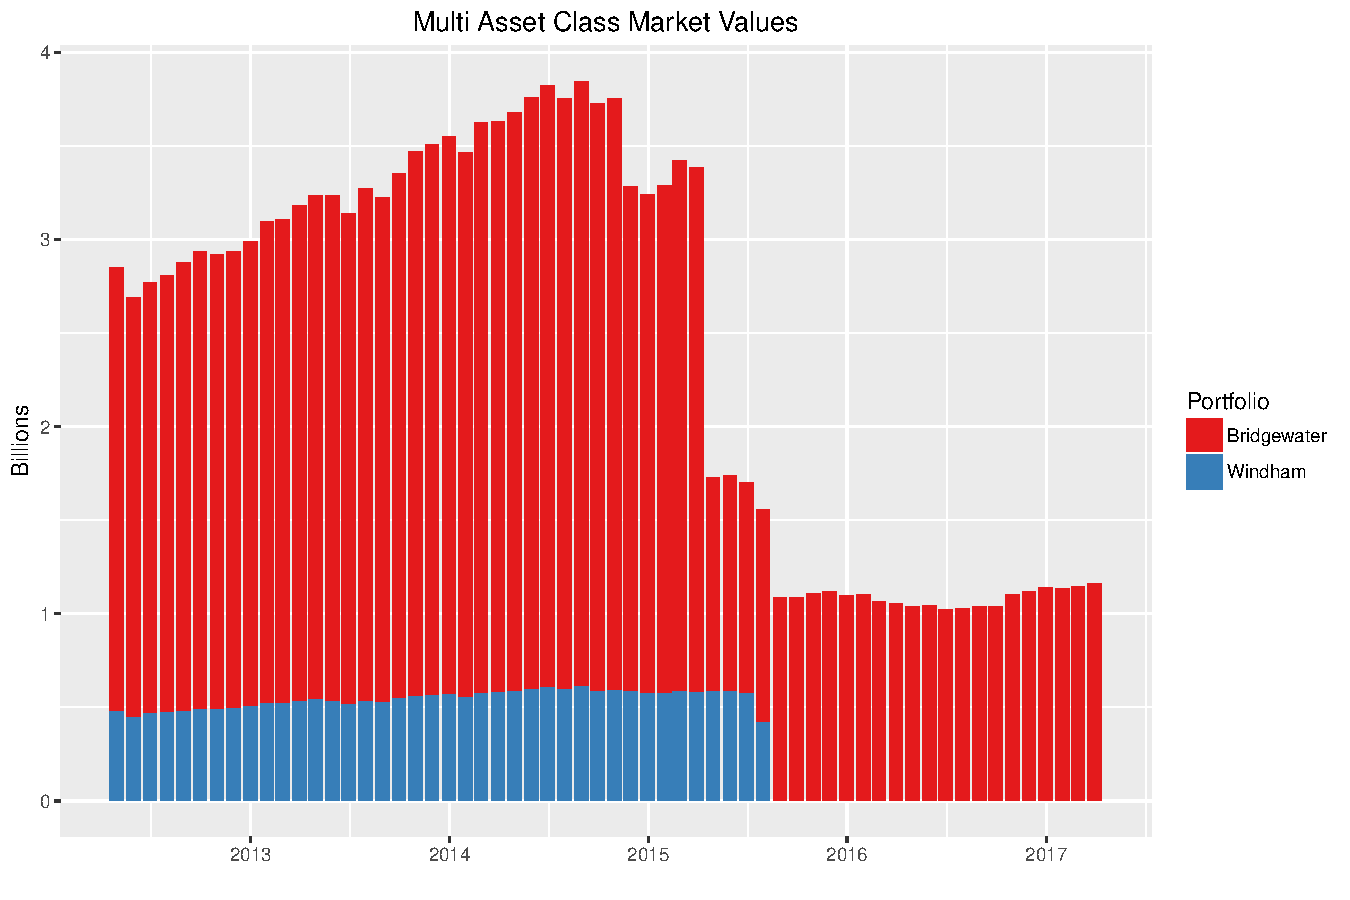
\includegraphics[width=\maxwidth]{figure/marketvalues-1} 

\end{knitrout}
\end{frame}
%
\begin{frame}[fragile]{Multi-Asset Class Performance}

\begin{knitrout}
\definecolor{shadecolor}{rgb}{0.969, 0.969, 0.969}\color{fgcolor}
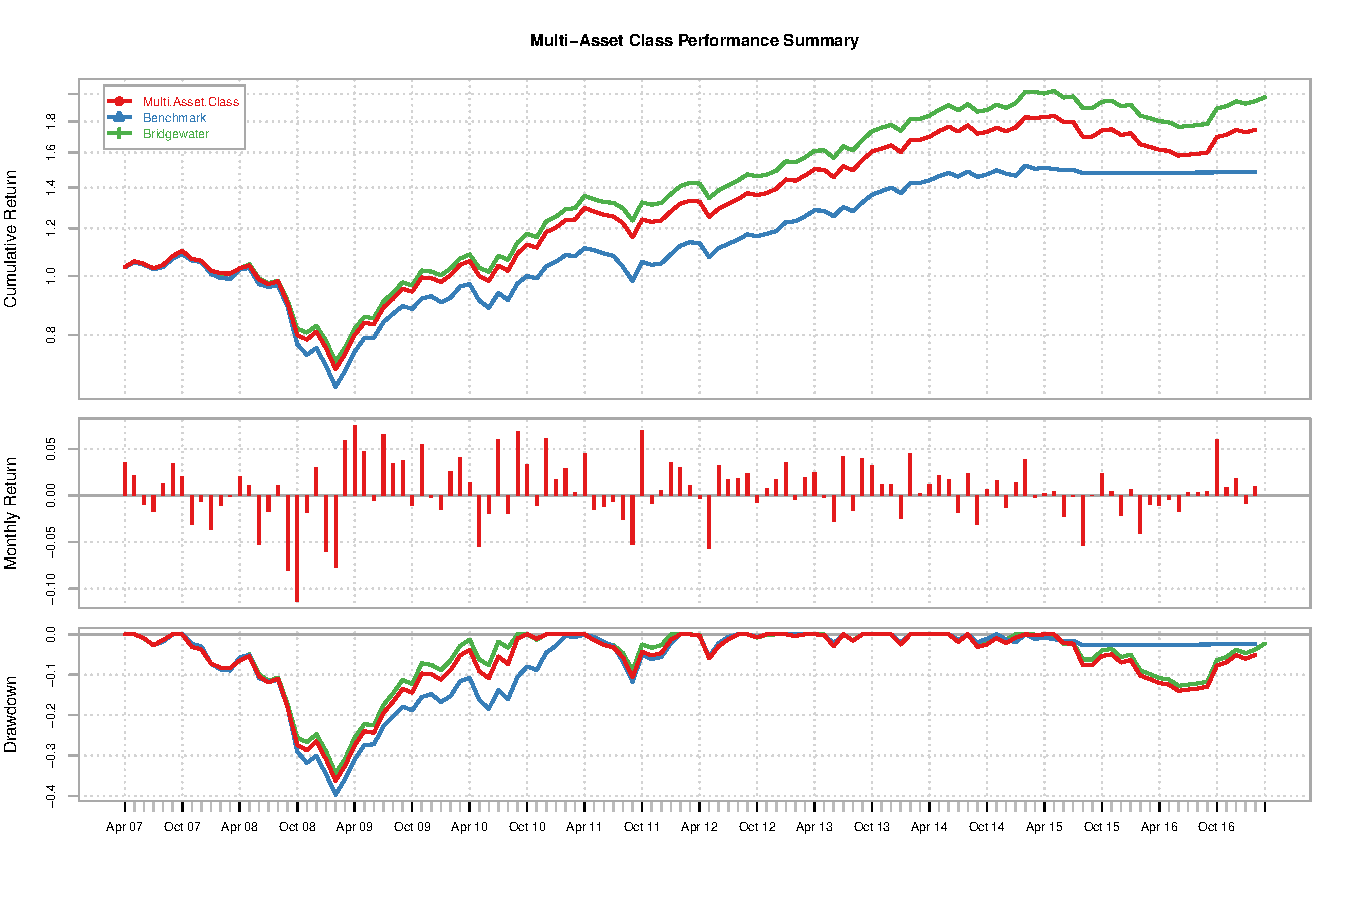
\includegraphics[width=\maxwidth]{figure/summary-1} 

\end{knitrout}
\end{frame}
%
\begin{frame}[fragile]{Bridgewater Performance}

\begin{knitrout}
\definecolor{shadecolor}{rgb}{0.969, 0.969, 0.969}\color{fgcolor}
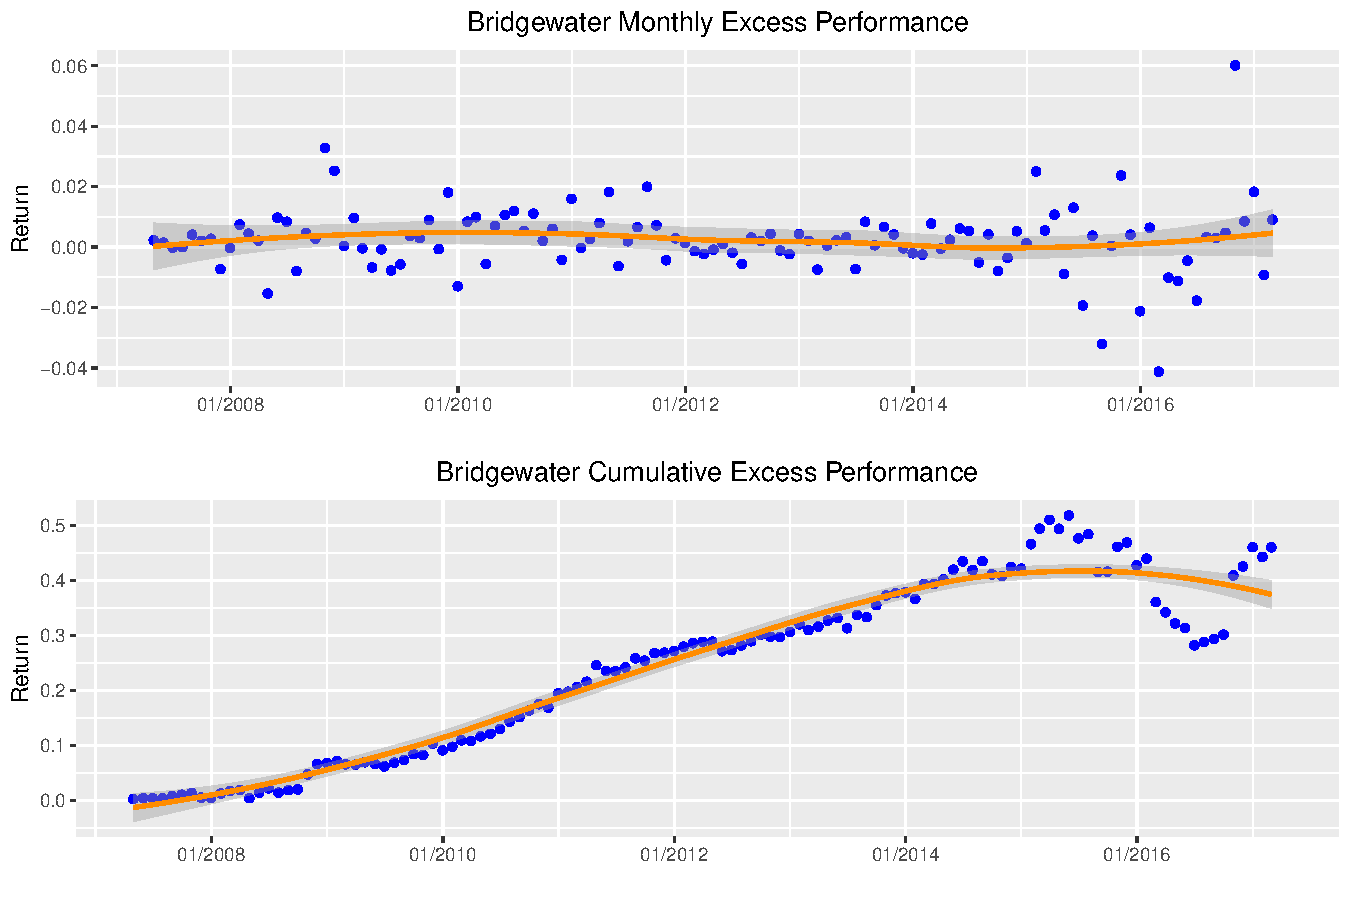
\includegraphics[width=\maxwidth]{figure/bw-1} 

\end{knitrout}
\end{frame}
%
\begin{frame}{Multi-Asset class Strategy Review Project}
\begin{itemize}
\item The Multi-Asset Class portfolio is currently under review.
\item ASRS retained Mercer Consulting to assist defining strategies that
may fit within the Multi-Asset Class. Mercer has helped develop criteria
for inclusion in the asset class, supplied portfolio data on risk
and return, and provided research notes on mangers that are highly
recommended.
\item TIMD has begun preliminary calls with candidates of interest, focusing
on each manager\textquoteright s investment process, portfolio construction
methodology.
\item Strategies that meet the ASRS search criteria and prove of interest
in preliminary calls will be subject to full due diligence of their
investment and operational capabilities.
\item IMD has not yet reached any conclusions on the recommendations as
a result of this process. 
\end{itemize}
\end{frame}
%

\end{document}
